%\documentclass[a4paper,man,natbib,donotrepeattitle]{apa6}
\documentclass[a4paper,doc,natbib,donotrepeattitle]{apa6}

\usepackage[english]{babel}
\usepackage[utf8x]{inputenc}
\usepackage{amsmath}
\usepackage{graphicx}
\usepackage[colorinlistoftodos]{todonotes}
\usepackage{times}
\raggedbottom %gets rid of unwanted space between paragraphs
\usepackage{float} %forces figures to appear in text
\usepackage{url} %formats urls in references so they wrap at text width
\usepackage{comment}
\usepackage{tabularx}
\usepackage{bm} %bold math


%\usepackage{caption}
%\captionsetup{justification=raggedright,
%              singlelinecheck=false}

\title{A General Architecture for Modeling the Dynamic Effects of Goals on Motivation and Decision Making}
\shorttitle{The GOAL Architecture}
\author{Timothy Ballard\textsuperscript{a}, Andrew Neal\textsuperscript{a}, Andrew Heathcote\textsuperscript{b}, Simon Farrell\textsuperscript{c}, Erin Lloyd\textsuperscript{a}, \& Jonathon Lim\textsuperscript{a}  (in some order)}
\affiliation{
\textsuperscript{a}The University of Queensland \linebreak
\textsuperscript{b}University of Tasmania
\linebreak
\textsuperscript{b}University of Western Australia
}



\abstract{}

\begin{document}
\maketitle

\section{A General Architecture for Modeling the Dynamic Effects of Goals on Motivation and Decision Making}

Every day, we are faced with the need to manage multiple, often competing, goals. In order to maximize the chances of achieving desirable outcomes and minimize the chances of incurring undesirable outcomes, we must constantly make decisions about which goals to prioritize, how much time to spend in pursuit of those goals, and when to divert our attention towards other goals. Successful goal management is, therefore, critical to our ability to function effectively \citep{Austin1996}. Yet humans are known to exhibit tendencies that undermine this ability. We procrastinate when deadlines are far off in the future, even if a significant amount of work needs be done \citep{Steel2006,Ariely2002}. We also fail to let go of goals toward which we've invested considerable time and effort, even when the prospect of successful goal achievement is slim \citep{Arkes1985,Olivola2018}. These tendencies can have serious consequences in safety-critical work contexts, such as aviation, medicine, or defense, where failure to effectively manage goals can lead to loss of life. For example, an air traffic controller who fails to successfully prioritize separation assurance goals among aircraft within their jurisdiction runs the risk of allowing a collision \citep{Hannah2014}.

Goal pursuit is an inherently dynamic process, where the motivational value of a goal changes over time as the person makes progress toward or away from the goal, and as deadlines draws nearer. Yet, although goals have long been a central construct in theories of motivation, and are increasingly being recognized as important for understanding decision-making, we know very little about how goal pursuit plays out over time. Theories of these dynamics tend to address only relatively specific aspects. For example, some theories consider how motivation changes as one makes progress toward the goal \citep{Carver1990,Bonezzi2011}. Other theories address the question of how motivation responds to a looming deadline \citep{Steel2006}. Still others focus on the relationship between motivation and goal difficulty \citep{Brehm1989,Wright2008}. To make matters even more complex, within these different theoretical microcosms, there are often competing accounts. For example the goal gradient hypothesis predicts that motivation increases as the goal becomes closer to being achieved \citep{Cryder2013,Hull1932}, whereas control theory predicts that motivation should decrease \citep{Carver1998,Powers1978}.

In an effort to refine our understanding of motivation and decision making, we introduce an integrated architecture, referred to as GOAL (goal oriented action linking), which describes the spatial and temporal dynamics of goal pursuit. We propose that the motivational value of a goal is influenced by three \textit{gradients}. The \textit{spatial} gradient reflects the component of motivation that is attributable to changes in the ``distance'' to the goal (i.e., the amount of progress needed to achieve it). The \textit{temporal} gradient reflects that contribution attributable to changes in the time to deadline. Finally, the \textit{spatiotemporal} gradient reflects the contribution attributable to the interaction between the distance to goal and time to deadline. In the next sections, we review the literature relevant to each gradient. At each step, we demonstrate how the relevant gradient is formalized within the GOAL architecture. We test the architecture in three experiments in which people make prioritization decisions whilst pursuing goals with varying distances and deadlines. We use hierarchical Bayesian modeling to examine the extent to which each gradient is influential when pursuing approach and avoidance goals.

% A goal is an internal representation of a desired or undesired state that serves as a reference point for evaluating behavior \citep{Austin1996,Carver1998,Neal}. Goals are important because they direct attention and guide the allocation of time and effort toward activities that promote goal attainment. However, at any given point in time, we often have several different goals that require attention. We therefore have to make choices about which goals to prioritize in order to maximize the chances of attaining desirable outcomes or prevent undesirable outcomes.

% AJH I found this term used once later in the document so added the definition below

%We use the term ``motivational potential'' to describe the degree to which a goal attracts resources such as attention, time, and effort at a given point in time. An examination into the dynamics of goal pursuit requires an understanding of the ways in which the environment changes over time, and the effects of these changes on a goal’s motivational potential. The two primary dimensions that characterize the state of the environment during goal pursuit are the distance to the goal (i.e., the amount of progress that needs to be made to achieve it) and the time to the deadline. We refer to the change in motivation attributable to changes in distance to the goal as the spatial gradient. We refer to the change in motivation attributable to changes in the time to deadline as the temporal gradient. Both gradients are influential during goal pursuit. For example, the goal gradient effect—the tendency for motivation to increase as a goal nears completion—arises due to the spatial gradient. Temporal discounting—the tendency for motivation to increase as a deadline looms—arises due to the temporal gradient. The problem is that most theories consider only one gradient (e.g., spatial: Carver \& Scheier, 1998\nocite{Carver1998}; Powers, 1973\nocite{Powers1973}; temporal:  Ainslie \& Haslam, 1992\nocite{Ainslie1992}; Steel \& König, 2006\nocite{Steel2006}) or treat the two gradients as equivalent (e.g., Trope \& Liberman, 2003\nocite{Trope2003}).


\section{The Spatial Gradient}

A goal is an internal representation of a desired or undesired state that serves as a reference point for evaluating behavior \citep{Austin1996,Carver1998,Neal}. The question of how the distance to a goal relates to an organism's motivation to move toward or away from it has a long history in a range of different disciplines within psychology. Yet there are differing perspectives regarding the answer to this question. The conflicting views can be broadly classified into one of two categories: \textit{proximity} versus \textit{discrepancy} perspectives. Proximity accounts propose that motivation derives from nearness to goal (e.g., the goal gradient hypothesis). Discrepancy accounts propose that motivation is the result of a discrepancy between oneself and a goal (e.g., control theory, social cognitive theory). In the following sections, we elaborate on each perspective.

\subsection{The Proximity Perspective}

Early theories of motivation proposed that goals have ``excitatory gradients'' that are determined by the positive and/or negative qualities that the goal possesses \cite[e.g.,][]{Lewin1935}. Positive qualities produce a tendency to approach the goal, whereas negative qualities produced the tendency to avoid it. The tendency to approach or avoid was proposed to increase as the organism becomes closer to the goal. The rationale for this hypothesis was that the reinforcement provided by the goal would be conditioned most strongly to the behavior that immediately preceded the goal being reached, and progressively weaker as the goal became more remote (Hull, 1932). The avoidance gradient was said to be steeper than the approach gradient, producing a higher maximum excitation level, but dropping off more quickly with distance to the goal. This set of propositions is known as the \textit{goal gradient hypothesis} \citep{Hull1938}.

Early tests of the goal gradient hypothesis were limited and almost exclusively conducted with rats \citep[e.g.,][]{Berg1942,Anderson1933,Weiss1960}. However, in the last decade there has been a resurgence in interest in examining the goal gradient hypothesis in humans. For example, \cite{Kivetz2006} demonstrated the participants in a cafe reward program purchased coffee more frequently when closer to reaching the number of purchases required to obtain a free coffee. They also showed that internet users who could earn reward certificates for rating a certain number of songs expended more time and effort when closer to their goal. \cite{Cryder2013} found that people were also sensitive to the goals of others. For example, charities receive more donations when closer to their fund-raising goals. The goal gradient effect has also been referred to as the ``goal looms larger'' effect \citep[e.g.,][]{Schmidt2007}.

Several different models have been used to capture these empirical effects. \cite{Kivetz2006} proposed a model, referred to as the goal-distance model, in which effort investment is a decreasing function of the ratio of the current distance to the goal to the original distance. \cite{Bonezzi2011} suggested that this behavior can also be explained by a model in which motivation is determined by the perceived marginal value of progress toward the goal, which increases as distance to the goal decreases. This latter explanation is equivalent to a hyperbolic model, where the perceived marginal benefit of moving one unit closer to the goal is equal to the proportion of the remaining distance that will be completed. Though formally different, both models share the assumption that motivation decreases monotonically with distance to the goal. This suggests that the spatial gradient should be negative.

Consistent with Hull's early predictions, there is some evidence that the goal gradient differs depending on whether a person is attempting to approach something desired or avoid something undesired. For example, \cite{Forster1998} presented participants with an anagram task in which the goal was to identify 90\% of all possible words. In the approach condition, while working on the anagrams participants had to press upward on a skin conductance machine attached to the underside of a table. In the avoidance condition, participants had to push downward on a machine located attached to the top of the table.
% AJH Not clear to me why this is avoidance and the other approach
They showed people applied more pressure as they became closer to finishing the anagrams and that this effect was stronger in the avoidance condition. Forster et al. interpreted this result as evidence that the avoidance gradient is steeper than the approach gradient. However, it is important to note that in this study the participants were not actually given avoidance goals. In both the approach and avoidance conditions, the anagram task was the same. Thus, the results should be interpreted with caution.
%TB - 4 July - This study is absolute crap. I'm debating whether to include it or not. The reason for including it is a) it's one of the few human studies that addresses avoidance and b) it's a good example of why we need better work in this area.

% AJH In that case if you keep it in play out these criticisms!

Although the goal gradient hypothesis has a long history, and is accumulating empirical support, there are many situations in which people behave in a way that violates this hypothesis. For example, when people evaluate their progress with respect to their initial state, as opposed to their goal state, effort investment can decrease as the goal nears \citep{Bonezzi2011}. Furthermore, the effects of distance to goal depend on changes in the expectancy of goal achievement \citep{Liberman2008}. When the perceived likelihood of achieving the goal increases beyond a certain point, movement toward a goal will likely lead people to divert attention elsewhere \citep{Louro2007}.
% AJH Dont get this
Further, when simultaneously managing multiple-goals, people often direct effort toward the goal that is furthest from attainment \citep{Schmidt2007,Ballard2017}. These observations suggest that the goal gradient hypothesis may not be sufficient to account for the complex effects of distance-to-goal on motivation, especially in environments where there is more than one goal.
% AJH added this clause in clarificaiton
In the next section, we therefore examine a competing perspective.

\subsection{The Discrepancy Perspective}

Another prominent perspective that provides insight into the relationship between distance to goal and motivation is the family of theories that derives from perceptual control theory \citep[control theory, for short;][]{Powers1973,Powers1978}. Control theory describes the dynamic interaction between a system (e.g., a person) and its environment as a discrepancy-reducing, negative feedback loop. The theory assumes that people regulate their behavior by monitoring the state of some variable in the environment and comparing it to a reference state (i.e., a goal). The presence of a discrepancy between the current state of the variable and the goal alerts the individual of the need to apply effort. This prompts the individual to take actions to reduce that discrepancy. This simple model of self-regulation has been highly influential in theoretical frameworks for understanding processes such as work motivation \citep[e.g.,][]{Klein1989,Lord1994,Carver1990,Jagacinski2003} and well-being \citep{Higgins1997,Trew2011}. The core assumption shared among control theory-derived frameworks is that motivation arises as the result of a discrepancy between one's goal and current state.

The assumption that people mobilize their effort in response to discrepancies has lead to the prediction that there should be a positive relationship between distance to a goal and the amount of effort or attention directed toward it, because longer distances signal a larger discrepancy to be corrected \citep[e.g.,][]{Deshon2005,Unsworth2009}. This prediction is in line with earlier work demonstrating that the magnitude of the discrepancy between one's goal and performance is positively related to subsequent effort \citep{Kernan1990,Campion1982}. More recently, the discrepancy perspective has been successful in explaining complex resource allocation process undertaken when pursuing multiple goals. In this context, people commonly direct their time and effort toward the goal with the largest discrepancy \citep{Schmidt2007,Schmidt2009,Schmidt2009a,Ballard2016c}. It should be noted that this work has almost exclusively addressed approach goals. Nevertheless, the evidence highlights the potential for a positive spatial gradient in the approach context.

Unlike the goal gradient hypothesis, control theory does not explicitly address avoidance goals. Some have argued on the basis of control theory that, when faced with an avoidance goal, individuals are motivated to enlarge the discrepancy \citep[e.g.,][]{Carver1998,Ballard2016c}. This argument suggests that motivation to avoid should decrease with increasing distance to the undesired state, which is the same prediction the goal gradient hypothesis makes regarding the avoidance context. This assumption is supported by a small number of studies, which have shown that people managing avoidance goals generally prioritize the whichever goal has the smallest discrepancy \citep{Ballard2016c,Ballard2016b,Ballard2018}.

\subsection{Modeling the Spatial Gradient}

The proximity and discrepancy perspectives make fundamentally different assumptions about the spatial gradient. They therefore generate unique predictions about the relationship between the distance to a goal, state, or object in the environment and the motivation to approach or avoid. The form of the spatial gradient within the GOAL architecture must, therefore, be sufficiently flexible to capture both perspectives. We model the spatial gradient as follows:

\begin{equation}
SG_{ij} =
\begin{cases}
D_{ij}^\delta, & \text{if } \delta >= 0 \\
(1-D_{ij}^{-\delta}), & \text{if } \delta < 0
\end{cases}
\label{SGequn}
\end{equation}

\noindent where $SG_{ij}$ is the level of the spatial gradient for goal $i$ and time $j$. $D_{ij}$ represents the distance to goal $i$ at time $j$. In our model fits $D_{ij}$ was scaled to be between 0 and 1, where 1 represents the maximum possible distance from the goal. The $\delta$ parameter controls the shape of the spatial gradient, and was constrained to fall between -1 and 1. When $\delta < 0$ the spatial gradient is negative, such that motivation decreases with distance to the goal. This assumption is consistent with early formalizations of the goal gradient hypothesis \citep[e.g.,][]{Hull1938}, which assumed that the rate of change in motivation decreased with increasing distance. When $\delta > 0$, the spatial gradient is positive, consistent with most discrepancy accounts \citep[e.g.,][]{Vancouver2005}. When $\delta$ is equal to either -1 or 1, the spatial gradient is linear. When $\delta$ falls between these values, the effect of distance to goal on motivation has diminishing returns. \citep[e.g.,][]{Kahneman1979}. Although other shapes are possible, such as increasing returns or non-monotonic effects of distance, we found the relatively simple formulation in Equation (\ref{SGequn}) was sufficient, and importantly aided model identifiability. In more complex cases \cite[e.g.,][]{Bonezzi2011}, mixtures of gradients of the form in Equation (\ref{SGequn}) with positive and negative parameters might be considered.

The predictions of proximity and discrepancy perspectives, as formalized by the GOAL architecture, are summarised in the first two panels in the top row of Figure \ref{fig:hypothetical_gradients}. In each panel in that row the x-axis represents the distance to a hypothetical (approach) goal and the y-axis represents the time to the deadline for that goal. The color of the surface represents the motivation value of the goal given the combination of distance to goal and time to deadline, and the gaps between successive vertical lines represent equal effects of a change in distance on the gradient. As can be seen, the proximity perspective assumes that motivation decreases as distance to the goal increases, but is unaffected by the time to the deadline. The discrepancy perspective assumes that motivation increases with distance to an approach goal (but decreases with distance to an avoidance goal), and is also unaffected by the time to the deadline.

\begin{figure}[h!]
\centering
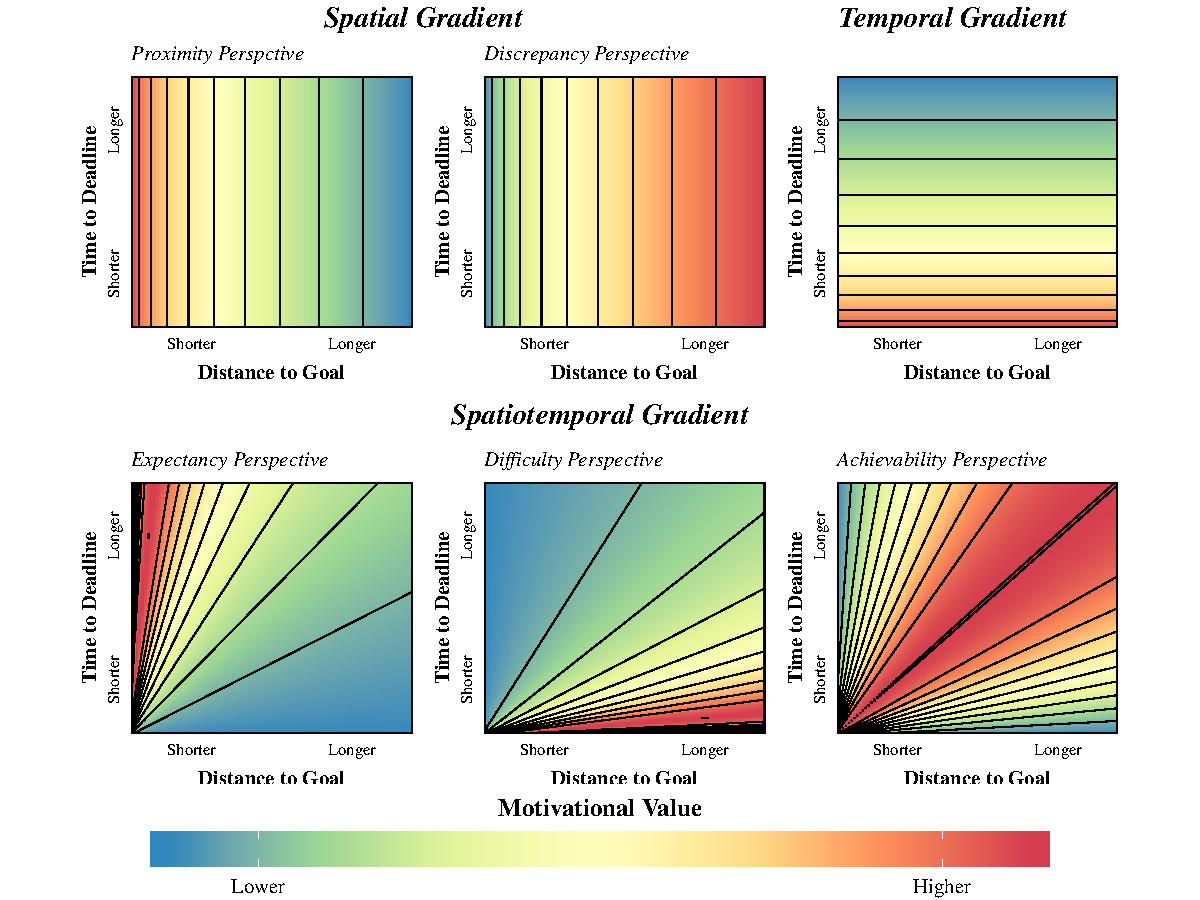
\includegraphics[width=1\textwidth]{hypothetical_gradients.pdf}
\caption{\label{fig:hypothetical_gradients} Summary of competing predictions regarding the spatial, temporal, and spatiotemporal gradients. In each panel, the x-axis represents the distance to a hypothetical goal and the y-axis represents the time to the deadline for that goal. The color of the surface represents the motivation value of the goal given the combination of distance to goal and time to deadline. Note that only predictions regarding approach goals are shown. For avoidance goals, the discrepancy, expectancy, and difficulty perspectives predict the opposite pattern to what is shown in the figure. }
\end{figure}


\section{The Temporal Gradient}

Although the the motivation literature has typically focused on the spatial dimension, much of what we know about the temporal properties of goals come from the decision making literature. In this literature, there is a large body of work that has attempted to understand discounting effects by studying intertemporal choice, which refers to the choice among outcomes that occur at different times \citep{Dai2014}. A typical paradigm in this literature involves asking participants to choose between two hypothetical monetary rewards: one that is smaller, but immediate and another that is larger, but delayed. For example, \cite{Murphy2001} used this paradigm to determine the immediately available reward amount that was subjectively equivalent to a delayed reward of \$500. As the delay for the \$500 reward increased, the immediate reward that participants were willing to accept instead of the \$500 decreased. Others have found that the preference for a smaller, short-term reward in favor of a larger, long-term reward reverses as the delays for both rewards increase \citep{Green1994,Kirby1995}. Temporal discounting has been found to vary by the size of the reward, with smaller rewards being discounted more strongly than larger amounts \citep{Estle2006}. It also varies according to whether outcomes are gains (i.e., rewards) or losses. There is evidence that delayed losses are discounted less strongly than delayed gains  %\citep{Goncalves2015}
\citep{Murphy2001,Goncalves2015}, although \cite{Estle2006} found this effect only for smaller amounts of money.

Temporal discounting has also been observed in non-monetary contexts. For example, \cite{Odum2003}, examined people's preferences for delayed vs. immediate food and alcohol. They found that discounting to be stronger for alcohol and food than they were for money. \cite{Bashir2014} argued that discounting effects may play a role in people's responses to climate change. They showed that framing the consequences of climate change as more temporally proximal increases engagement in environmentally friendly behavior.

Although temporal discounting has typically been studied in paradigms involving static, one-shot decisions, it is likely also influential in more dynamic decision making environments like those encountered during goal pursuit. When pursuing a goal, the individual must make a series of interdependent decisions involving which goal to prioritize, how much effort to exert in pursuit of the goal, and when to shift focus elsewhere. Decisions during goal pursuit have downstream effects because they shape the environment in which future choices are made. For example, the decision to spend a day procrastinating instead of working on a grant application means that more work will have to be done in subsequent days. In this type of environment, the perceived value of goal achievement (e.g., the reward for successfully completing the application) influences the decisions that are made at each step in the process \citep{Ballard2018}. Yet longer deadlines often mean that more time must pass before the rewards associated with goal achievement can be obtained. This can lead the perceived value of goal achievement to be subject to the effects of temporal discounting. In other words, all else being equal, the reward associated with achieving a goal (or the punishment associated with goal failure) should be more salient when the deadline determining whether the goal has been achieved or failed is nearer. These arguments suggest that the temporal gradient should be negative.

\subsection{Modeling the Temporal Gradient}

The GOAL architecture assumes that the temporal gradient has the same functional form as the spatial gradient, so it is scaled similarly and so both can be enter into the GOAL architecture via a simple additive combination:

\begin{equation}
TG_{ij} =
\begin{cases}
T_{ij}^\tau, & \text{if } \tau >= 0 \\
(1-T_{ij}^{-\tau}), & \text{if } \tau < 0
\end{cases}
\end{equation}

\noindent where $TG_{ij}$ is the level of the temporal gradient for goal $i$ and time $j$. $T_{ij}$ is time remaining before the deadline for goal $i$ at time $j$. The $\tau$ parameter controls that shape of the temporal gradient. We assume that $\tau$ is negative, meaning the motivation decreases with longer deadlines. This assumption is consistent with hyperbolic discounting models of intertemporal choice and motivation \citep[e.g.,][]{Ainslie1975,Steel2006}. As can be seen in the top-right panel of Figure \ref{fig:hypothetical_gradients}, the arguments relating to the temporal gradient lead to the prediction that motivation should increase as the deadline for goal achievement becomes nearer.

\section{The Spatiotemporal Gradient}

The spatial and temporal gradients represent the independent effects of distance to goal and time to deadline on a goal's motivational value. Yet the spatial and temporal gradients are sometimes not independent. Several theories suggest that the motivation is influenced by the difficulty of goal achievement in ways that are not naturally represented by a simple additive combination of separate spatial and temporal gradients.

Although these accounts do not explicitly address the effects of distance to goal and time to deadline, the existence of a relationship between goal difficulty and motivation suggests that people combine information about distance and time. This is because goal difficulty is a function of both the amount of progress required to reach the goal (i.e., distance) and the amount of time available before the deadline. We therefore propose a third gradient, which we refer to as the spatiotemporal gradient, to account for non-additive effects. The spatiotemporal gradient represents changes in motivation attributable to changes in the relationship between distance and time during goal pursuit. In the following subsections, we describe three different perspectives that can be used to derive predictions regarding the effects of the spatiotemporal gradient: the expectancy perspective, the difficulty perspective, and the achievability perspective.

\subsection{The Expectancy Perspective}

Expectancy is a construct that has played a central role in theories of motivation and decision making \citep{Vroom1964,Bandura1977}. Within the motivation literature, expectancy has been generally defined as the belief that effort will result in a desired outcome (e.g., reaching an approach goal or not reaching an avoidance goal). Expectancy has been identified as a key factor in determining the investment of effort, with the assumption being that increasing expectancy will increase effort application \citep{Locke1990,Bandura1977,Vroom1964,Steel2006}. Expectancy is also an important element in theories of economic decision making \citep[e.g.,][]{vonNeumann1947,Luce1957}, where it has been defined as the subjective likelihood of an outcome occurring. These theories assume that the expectancy of a favorable outcome increases the likelihood of selecting a particular course of action. These arguments collectively suggest that the expectancy of achieving a goal should play an important role during goal pursuit.

Evaluating the expectancy of goal achievement requires consideration of both distance and time. When pursuing an approach goal, the farther one is from the goal, the more effort must be invested in order to achieve it. Thus, all else being equal, expectancy should decrease with distance \citep{Liberman2008}. Yet the expectancy of achieving an approach goal is also influenced by deadlines. The more time a person has available, the easier it is to reach the goal. Thus, expectancy should increase with the amount of time available \citep{Vancouver2010}. A simple way to represent expectancy is as the ratio of the time to deadline to the distance to goal. This ratio reflects the rate of progress that is required to reach the goal, which determines how difficult the goal is to achieve. According to this instantiation of the expectancy perspective, the lower the rate of progress required to reach an approach goal, the lower the expectancy of achieving it.


% AJH An argueably simpler one is Distance - Time, which is just what the ratio is on a log scale, i.e., log(Distance/Time) = log(Distance) - log(Time). Where does this ratio idea come from and why is it better that additive? It doesn't have to be better, just wondered ... Maybe the simplest way to reword here is "A simple way to go beyond an additive model (i.e., expectancy = time - distance) is the ratio ....

The expectancy of achieving an avoidance goal, by contrast, should increase with distance to the goal as the person moves further from the undesired state that they are attempting avoid. Expectancy should also decrease with the amount of time available because longer deadlines mean that more time and effort must be spent avoiding the undesired state. Thus, according to this interactive expectancy perspective, the strength of motivation to pursue an avoidance goal should decrease with the ratio of the time to the deadline to the distance to the goal.

\subsection{The Difficulty Perspective}

The expectancy perspective treats the allocation of effort as a proactive process, whereby the person chooses courses of action that they evaluate as being likely to pay off. An opposing view is that effort is allocated in a compensatory manner. Information processing models \citep{Hendy1997,Hockey1997} propose that effort is a scarce resource, and that the application of effort is costly. As a result, people seek to minimize effort, applying only the amount that is required to meet the demands imposed by the situation \citep{Kool2010,Westbrook2015}.

Support for this argument can be found in several different areas. For example, studies of effort discounting have shown that people people are willing to apply more effort to obtain larger rewards \citep{Libedinsky2013,Westbrook2013}. Studies of time pressure have shown that people work harder when they have less time to complete a task \citep{Bryan1967,Latham1975,Peters1984}. Finally, research in the human factors literature has revealed that workload increases with the ratio of the time required to complete a task to the time available \citep{Hendy1997}.

If effort is used as a compensatory resource during goal pursuit, then motivation should increase with the difficulty of goal achievement. Difficulty can, therefore, be conceptualized as the inverse of expectancy. For approach goals, difficulty increases with the distance to the goal and decrease with the time available. Thus, the difficulty of achieving an approach goal can be represented as the ratio of the distance to goal to the time available. According to the difficulty perspective, the motivational value of pursuing an approach goal should increase with this ratio. For avoidance goals, difficulty decreases with distance and increases with the time available. Thus, the strength of motivation to pursue an avoidance goal should decrease with the ratio of the distance to the goal to the time to the deadline.


\subsection{The Achievability Perspective}

Although the expectancy and difficulty perspectives are well-established, critics have suggested that neither is sufficient to account for the complex dynamics of motivation during goal pursuit. For example, although expectancy is likely to be influential, if a task is too easy, people will often divert resources to other tasks where time and effort are needed more \citep{Carver1998,Louro2007}. This behavior violates the expectancy perspective. On the other hand, if a goal is too hard to achieve, people are likely to give up \citep{Schmidt2009,Vancouver2010}. This behavior violates the difficulty perspective. These arguments highlight the need to consider a third perspective regarding the nature of the spatiotemporal gradient.

The third perspective proposes that the influence of difficulty and expectancy on motivation is non-monotonic. We refer to this account as the achievability perspective. It dates back to Atkinson's work on achievement motivation \citep[e.g.,][]{Atkinson1970}, which proposed that this relationship has an inverted u-shape, where motivation is highest when difficulty and expectancy are moderate and lowest when either difficulty is very low (and therefore expectancy is very high) or very high (and therefore expectancy is very low). Others have proposed a discontinuous relationship, where the intensity of motivation increases with difficulty up to the point where the individual decides that the goal cannot be achieved or that it is not worth the effort. When difficulty exceeds this level, the motivation to exert effort towards achieving the goal drops to zero \citep{Brehm1989,Kukla1972,Kruschke2012,Wright2008}. Though the inverted-u and discontinuous models are difficult to differentiate empirically, there is broad support for a non-monotonic relationship between difficulty or expectancy and motivation \citep[e.g.,][]{Wright1986,Karabenick1968,Biner1987,Brehm1983,Vancouver2008}. For example, \cite{Louro2007} found that dieters striving for weight loss goals allocated more effort to the goal when they had a moderate expectancy of achieving it than when they had either a low or a high expectancy.

If the relationship between difficulty, expectancy, and a goal's motivational value (i.e., the degree to which it attracts resources such as attention, time, and effort) is non-monotonic, motivation should be highest when the ratio of distance to time (or vice versa) is moderate, and lower when the value of this ratio is too low or too high. In the next subsection, we demonstrate how all three of these perspectives can accounted for in the GOAL architecture.

\subsection{Modeling the Spatiotemporal Gradient}

The model of the spatiotemporal gradient in the GOAL architecture must be sufficiently flexible to account for a non-monotonic relationship between the ratio of the distance to the goal to the time to the deadline and motivation. The specific functional form we assume is motivated by the need to place the spatiotemporal gradient on a similar scale to the temporal and spatial gradients so that all three can be combined additively:

\begin{equation}
STG_{ij} = \beta\Bigg[\frac{\alpha T_{ij}}{D_{ij}} + \frac{(1-\alpha) D_{ij}}{T_{ij}}\Bigg]^{-1},
\end{equation}

\noindent where $STG_{ij}$ is the level of the spatiotemporal gradient for goal $i$ at time $j$. The $\alpha$ parameter that takes on a value of between 0 and 1 and controls the shape of that gradient. When $\alpha = 0$ the strength of the spatiotemporal gradient increases linearly with expectancy (consistent with the expectancy perspective). When $\alpha = 1$ the strength of the gradient increases linearly with difficulty (consistent with the difficulty perspective). When $\alpha$ is between 0 and 1, the spatiotemporal gradient is non-monotonic and strongest at moderate levels of expectancy and difficulty (consistent with the non-monotonic perspective). When $\alpha = 0.5$, the spatiotemporal gradient reaches its maximum when $D_{ij} = T_{ij}$. The $\beta$ parameter scales the function so that it has a maximum value of 1, which puts it on the same scale as the spatial and temporal gradients. Without this parameter, the maximum height of the gradient would vary as a function of $\alpha$. $\beta$ is calculated as follows:

\begin{equation}
\beta = 2(1-\alpha) \sqrt{\frac{\alpha}{1-\alpha}} .
\end{equation}

The competing predictions regarding the expectancy, difficulty, and the non-monotonic perspective are summarized in the bottom row of Figure \ref{fig:hypothetical_gradients}. As can be seen, all three perspectives assume that motivation changes with the ratio of distance to time. The expectancy perspective assumes that motivation to pursue an approach goal is highest when there is a lot of time remaining and only a small distance to cover before the goal is reached.  The difficulty perspective assumes that motivation to pursue an approach goal is highest when there is little time remaining and a lot of distance to cover. Both perspectives predict the opposite relationships for avoidance goals (not shown in the figure). The achievability perspective assumes that motivation is highest when the time remaining before the deadline and the distance to the goal are approximately equal, which makes the goal moderately difficult to achieve.

\section{Putting it all Together}

To summarize the information presented thus far, the GOAL architecture is a framework for modeling the dynamics of motivation during goal pursuit. The architecture assumes that changes in motivation are attributable to changes in position along three gradients. The spatial gradient represents the changes in motivation that are attributable to changes in the distance to the goal (i.e., the amount of progress needed before the goal is reached). The temporal gradient represents the changes in motivation that are attributable to changes in the amount of time before the deadline that determines whether the goal has been achieved or failed. The spatiotemporal gradient represents the changes in motivation that are attributable to changes in the ratio of the distance to the goal to the time available before the deadline (which equates to the rate of progress required to reach the goal).

The GOAL architecture assumes that the spatial, temporal, and spatiotemporal gradients combine to influence the motivational value of goal $i$ at time $j$ (denoted $M_{ij}$). Specifically, we assume that the motivational value is determined according to a simple weighted additive equation:

\begin{equation}
M_{ij} = w_{1}SG_{ij} + w_{2}TG_{ij} + w_{3}STG_{ij},
\end{equation}

\noindent where $w_1$, $w_2$, and $w_3$ are weight parameters that determine the influence of the spatial, temporal, and spatiotemporal gradients respectively on motivation. We assume that $w_{1}$, $w_{2}$, and $w_{3}$ sum to one. These weights reflect the relative importance of each gradient in influencing the extent to which a person is motivated to prioritize a goal.

 In the sections that follow, we compare the six theoretical perspectives described above by using the GOAL architecture to quantify each gradient based on the data from three experiments. The aim is to examine whether any one perspective is sufficient to account for changes in motivation during goal pursuit in its own right, or whether more than one perspective must be integrated in order to account for the full complexity these effects.

Many have argued that the dynamics of goal pursuit cannot be examined by considering a single goal in isolation, because the motivational value of a goal is only influential when allocating resources toward a goal involves a cost to other goals \citep[e.g.,][]{Austin1996}. We therefore use a revealed preference paradigm \citep[e.g.,][]{Kool2014,Kool2010}, where participants make choices about which of two goals to prioritize. We measure motivation as the tendency to prioritize a particular goal. In order to generate predictions about which goal will be prioritized, we use a logistic choice model to transform the difference in motivational values into a set of choice probabilities. Specifically, the probability of prioritizing Goal A at time \textit{j} is calculated as follows:

\begin{equation}
pr_{A,j} = \frac{1}{1 + exp[-\theta(M_{A,j} - M_{B,j})]},
\end{equation}

\noindent where $\theta$ is a scaling parameter that represents sensitivity to the difference in motivational values. The probability of prioritizing Goal B is one minus the probability of prioritizing Goal A.

In Experiment 1, we manipulated the distance to each goal at the start of each goal pursuit episode, while holding the deadline constant between goals. In Experiment 2, we manipulated the time to deadline for each goal, while holding the starting distance constant. In Experiment 3, we manipulated both the starting distance and the deadline. In each experiment, we also manipulated goal type, such that participants sometimes pursued two approach goals and other times pursued two avoidance goals. As we used the same paradigm in all three experiments, we report the method for the three experiments together in this section. We then report the results from all three experiments together in the next section.




% AJH in propritonal forms one weight is determined by the others, cant recall if that is the case here, but a form like S*(W1*SG + W2*TG + W3* STG) where W1=w1/(w1+w2+w3), W2=w2/(w1+w2+w3) W3=1-W1-W2, where W1,W2,W3 <= 1 and S takes care of (often uninteresting) scaling issues. This is often the most informative from as the Wi have a direct interpretation as relative importance.



\subsection{Participants}

The full sample consisted of 330 participants. Participants in Experiments 1 and 2 were undergraduates at the University of Queensland who took part in exchange for course credit. Experiment 1 consisted of 146 participants (57\% female, 43\% male) with ages ranging from 17 to 51 years (M = 20.26, SD = 5.53). Experiment 2 consisted of 130 participants (60\% female, 40\% male) with ages ranging from 17 to 50 years (M = 19.93, SD = 5.01). Participants in Experiment 3 were members of the University of Queensland local community who received \$20 for taking part. Experiment 3 consisted of 54 participants (39\% female, 61\% male) with ages ranging from 18 to 40 years (M = 22.41, SD = 3.45). A total of 36 participants were excluded from the analysis because they did not finish the study (16 from Experiment 1, 16 from Experiment 2, and 4 from Experiment 3). This left final samples of 130, 114, and 50 participants for Experiments 1, 2, and 3 respectively. \footnote{Due to a technical error, approximately 3\% of the observations in Experiments 1 and 2 were not recorded. The missingness of the data was not systematically related to any of the experimental manipulations.}.

\subsection{Experimental Paradigm}
	We used an online farm simulation task to design an experiment suitable for testing the GOAL architecture. The task was broken down into a series of trials, which each represented an independent goal pursuit episode. In each trial, participants had to simultaneously manage either two crops (in the approach condition) or two weeds (in the avoidance condition). Each trial was broken down into a series of stages, which each represented a decision point in the growing season. In each stage, the participant had to make a decision about which crop or weed to treat at that point in time. Treating a crop encouraged its growth whereas treating a weed suppressed its growth.

\subsubsection{Approach Condition}In approach trials, participants had to manage two out of three possible crops (wheat, corn, or rice). Their objective was to ensure that the height of each crop was above the threshold height by the end the crop's growing season. At each stage in the growing season, participants had to choose which crop to treat. Treating a crop increased its potential for growth in that stage. Thus, on any given day, the treated crop would grow more on average than the neglected crop.

\subsubsection{Avoidance Condition}In avoidance trials, participants had to manage two out of three possible weeds (thistle, nettle, or lantana). Their objective was to ensure that the height of each weed was below the threshold height by the end the weed's growing season. On each day of the growing season, participants had to choose which weed to treat. Treating a weed suppressed its potential for growth on that day. Thus, on any given day, the treated weed would grow less on average than the neglected weed.

\subsection{Design}

In all three experiments, goal type was manipulated within participants, but was held constant across the two goals in each trial. That is, there were no trials in which participants had to simultaneously manage one approach and one avoidance goal.

\subsubsection{Experiment 1}

In this experiment, we also manipulated the difference between the height of the crop and the threshold height at the start of each trial (i.e., starting distance). The threshold height was always 240 cm. The combination of starting distances was manipulated within participants. We varied the starting distance for each goal across 7 levels (30, 45, 67.5, 90, 112.5, 135, or 150 cm), and including only the non-redundant combinations of distances (e.g., a distance of 30 for Goal A and 45 for Goal B is redundant with a distance of 45 for Goal A and 30 for Goal B). This manipulation resulted in 28 unique starting distance combinations and so the design had 56 unique experimental conditions (2 Goal Type X 28 Starting Distance Combination). Increasing the starting distance made approach goals harder to achieve, but avoidance goals easier to achieve. However, the overall difficulty of the task was constant across goal type conditions because an approach goal with a starting distance of 30 cm was equally easy to achieve as an avoidance goal with a starting distance of 150 cm, an approach goal with a starting distance of 45 cm was equally easy to achieve as an avoidance goal with a starting distance of 135 cm, and so on.

In this experiment, participants were told that each stage in the trial represented one day in the growing season. The growing season for each crop/weed was always 30 days. In the approach condition, the growth of the crop that the participant chose to treat on that day was determined by sampling from a normal distribution with a mean of 6 cm and a standard deviation of 3 cm. The growth of the neglected crop was determined by sampling from a normal distribution with a mean of 0 cm and a standard deviation of 3 cm. In the avoidance condition, the growth of the weed that the participant chose to treat on that day was determined by sampling from a normal distribution with a mean of 0 cm and a standard deviation of 3 cm. The growth of the neglected weed was determined by sampling from a normal distribution with a mean of 6 cm and a standard deviation of 3 cm.

\subsubsection{Experiment 2}

Experiment 2 was identical to Experiment 1 except that starting distance was held constant and deadline was manipulated within participants. All crops/weeds started at a height of 90 cm below the threshold (i.e., the starting distance was always 90 cm). Deadline was manipulated in a similar manner to starting distance in Experiment 1 by varying the length of the growing season for each crop/weed across 7 levels (18, 20, 24, 30, 40, 60, or 90 days) and including only the non-redundant combinations of deadlines. This design produced 56 unique experimental conditions (2 Goal Type X 28 Deadline Combination). Increasing the deadline made approach goals easier to achieve because there were more opportunities for growth. For the same reason, increasing the deadline made avoidance goals harder to achieve. However, the overall difficulty of the task was constant because achieving an approach goal with a deadline of 90 was approximately the same in difficulty as achieving an avoidance goal with a deadline of 18, and so on. The deadline manipulation also produced trials that were approximately equal in difficulty to the trials produced by the starting distance manipulation in Experiment 1.

\subsubsection{Experiment 3}

In this experiment, we manipulated both starting distance and deadline within participants, and so more trials were required than in Experiments 1 and 2. In order to accommodate the extra trials, we reduced the number of decisions per trial so that no more than 8 decision stages were included any trial. Participants were told that each decision stage represented one month in the growing season.  We varied the length of the growing season across 4 levels (1, 2, 4, or 8 months) and the starting distance for each goal across 4 levels (10, 20, 40 or 80 cm). The threshold height was always 200 cm in this experiment. As with Experiments 1 and 2, we included only non-redundant cells in the design. These manipulations resulted in 120 unique starting distance x deadline combinations, and so the design had 240 unique experimental conditions (120 approach trials and 120 avoidance trials).

In the approach condition, the growth of the crop that the participant chose to treat was determined by sampling from a normal distribution with a mean of 20 cm and a standard deviation of 20 cm. The growth of the neglected crop was determined by sampling from a normal distribution with a mean of 0 cm and a standard deviation of 20 cm. In the avoidance condition, the growth of the weed that the participant chose to treat was determined by sampling from a normal distribution with a mean of 0 cm and a standard deviation of 20 cm. The growth of the neglected weed was determined by sampling from a normal distribution with a mean of 20 cm and a standard deviation of 20 cm.

\subsection{Procedure}

Upon starting the experiment, participants were first presented with computerized task instructions. They then completed a series of practice trials. Participants then completed each unique experimental condition. In Experiments 1 and 2, the 56 unique conditions were completed in random order. In Experiment 3, the approach and avoidance conditions were blocked such that participants either completed all approach trials first or all avoidance trials first (with the order of trials randomised within each block). In each trial, the position of the crop or weed on the screen (i.e., left vs right) was randomly determined, as well as the type of crop or weed that the participant encountered. Participant treated the left crop/weed by pressing the \textit{a} key and the right crop/weed by pressing the \textit{k} key. After they selected a treatment, the task would immediately update to the next decision stage, so that the participant could see how much the height of each crop or weed had changed and make the next treatment decision. The heights of the crops/weeds, the threshold height, and the number of days/months left in each growing season were displayed on the screen throughout the trial.

For trials where the crops/weeds being treated had the same growing season, the trial ended when the growing season finished. For trials where the crops/weeds did not have the same growing season, the trial ended when the longer growing season finished. In these trials, the crop or weed with the growing season that finished earlier was replaced by a new crop/weed after its growing season ended. These replacements were required to ensure that the participant still had to make prioritization decisions after the first deadline was reached. The starting distance for the replacement crops or weeds was always equal to 3 times the number of days/months remaining in the other growing season, which ensured that the new goal was moderately difficult to achieve.

\section{Behavioural Results}

We begin our presentation of the results by describing the patterns of choices made by participants in the three experiments. In order to facilitate interpretation and avoid repetition, we combined the results across the three experiments. Where relevant, we have provided the figures with the results broken down by experiment in the supplementary material, which can be found (INSERT OSF LINK). We use vector field plots to illustrate how goal prioritization decisions were influenced by the combination of distance to goal and time to deadline for each of the two goals being pursued (see Figure \ref{fig:descriptives}). The distance to goal (D) and time to deadline (T) variables were converted to the 0-1 scale assumed by the GOAL architecture by dividing the raw value of that variable by 1 + the maximum value observed in the experiments (for distance, 187 cm; for deadline, 90 days in Experiments 1 and 2 and 8 months in Experiment 3). The time to deadline for each goal is broken up into three ranges (< .25, 0.25 - 0.5 and > 0.5) and mapped to different panels (so 9 each for approach and avoidance), with the columns representing the time to deadline for the right-hand goal and the rows representing the time to deadline for the left-hand goal. The distance to the right- and left-hand goal is represented on the x- and y- axes, respectively, of each panel. The yellow lines at $D = 0$ indicate the threshold that determines whether the goal is achieved or failed. The horizontal line indicates the threshold for the left-hand goal and the vertical line indicates the threshold for the right-hand goal. Distance was broken up into a finer set by rounding to the nearest tenth, so each panel consists of 121 possible cells. Results in each cell are represented by a vector where there were a sufficiently large number of observations ($N >= 10$). The orientation of the vector indicates the average direction which the participants choose to move. The upward component of each vector indicate choices that decrease the distance to the goal on the left whereas the rightward vector component indicates choices that decrease the distance to the goal on the right. Hence, vectors pointing up indicate choices preferencing the left goal, vectors pointing right indicate choices preferencing the right goal and vectors along the diagonal indicate decisions preferencing both goals equally.

% AJH would be nice to reword the caption to not be identical to text (apart from the last sentence). You have not defined what a "cell" is. From counting arrows I figure you also dicreteized distance 0-0.1,0.1-0.2 ... 0.9-1 so I wrote that above.

%TB - Okay, I've added a description about how distance was discretized. And I've shortened the figure caption and have referred the reader to the text for more info.

\begin{figure}[h!]
\centering
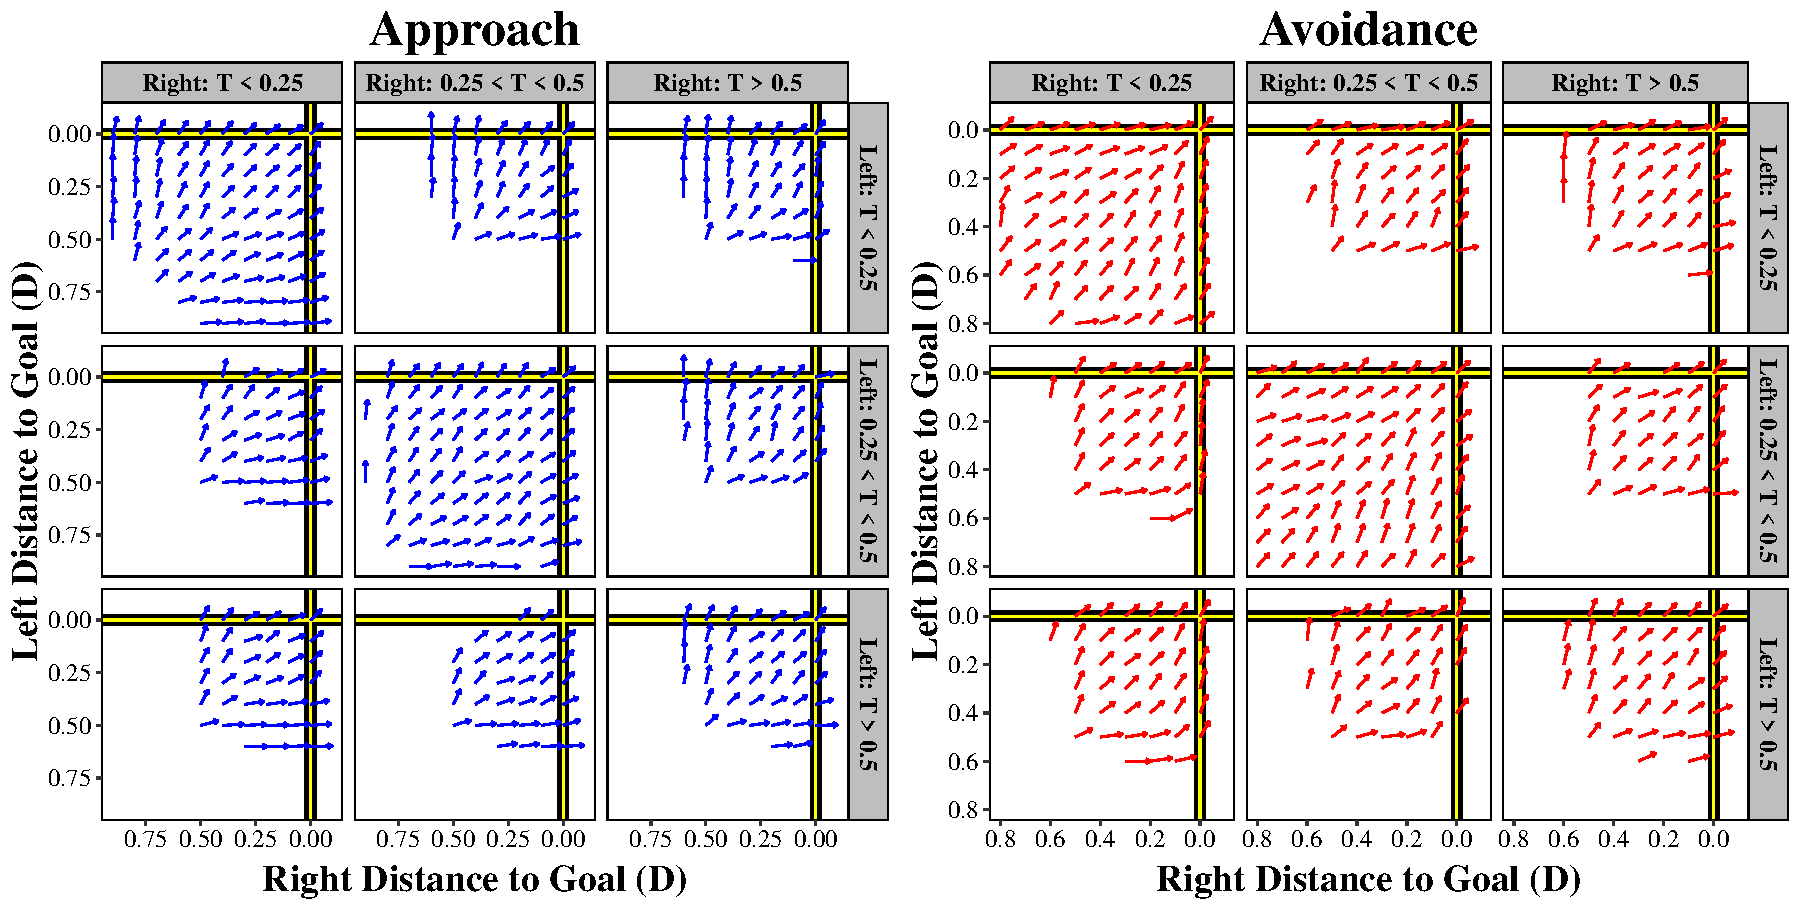
\includegraphics[width=1\textwidth]{descriptive_gradient.pdf}
\caption{\label{fig:descriptives} Vector field plots illustrating the influence of distance to goal, time to deadline, and goal type on prioritization decisions across the three experiments. The time to deadline for each goal is broken up into the different panels, with the columns representing the time to deadline for the right-hand goal and rows representing the time to deadline for the left-hand goal. The distance to the right- and left-hand goal is expressed on the x and y axes respectively. The yellow lines at $D = 0$ indicate the threshold that determines whether the goal is achieved or failed. The orientation of the vector indicates the direction which the participants choose to move through the field. Note that only cells containing 10 or more observations are shown. See text for more detail.}
\end{figure}

\subsection{Approach Condition}
The results for the approach condition (the left set of panels) suggest that goal prioritization decisions vary depending on the combination of distance to goal and time to deadline for each goal. Consider the top-left panel, where the time to both deadlines is relatively short. Under these conditions, people tend to prioritize whichever goal is closer to being achieved. This can be seen by the fact that the vectors above the diagonal, which indicate states in which the left-hand goal is closer to being achieved, tend to point upward. Vectors below the diagonal, which indicate states in which the right-hand goal is closer to being achieved, point rightward. Consider now the middle and bottom-right panels. In these panels, the deadlines are longer, but are still similar between the two goals. There, the tendency to prioritize the goal that is closer to being achieved is weaker. This can be seen by the fact that there are fewer arrows pointing directly upward or rightward and more arrows pointing diagonally toward the top-right corner of the panel (indicating that goals are being equally prioritized).

Consider now the top-middle, top-right, and middle-right panels. In these panels, the deadline for the left-hand goal is shorter than the deadline for the right-hand goal. In this scenario, there is a stronger tendency to prioritize the left-hand goal (i.e., the arrows tend to point more upward than rightward). The opposite is true in scenarios where the deadline for the right-hand goal is shorter (the middle-left, bottom-left, and bottom-middle panels). Here, the results suggest a tendency to prioritize the right-hand goal (i.e., the arrows tend to point more rightward than upward). These results together suggest that distance to goal and time to deadline exert complex effects on motivation when pursuing approach goals. Specifically, when goals have different deadlines, people tend to be more motivated to prioritize the goal with the shorter deadline. When goals both have relatively short deadlines, people tend to be more motivated to prioritize the goal that is closer to being achieved. When goals both have longer deadlines, the overall preference for prioritizing a particular goal is less clear.

\subsection{Avoidance Condition}
The results for the avoidance condition (the right set of panels) suggest a much simpler pattern of choices. In the avoidance condition, people tend to make choices that allow them to maintain their distance from the undesired threshold that is closer to being reached. As a result of these decisions, they tend to move closer to the undesired threshold that is farther from being reached. This can be seen by the fact that the vectors tend to point inward toward the diagonal of each panel. In contrast to the approach context, motivation when pursuing avoidance goals appears to be much less strongly affected by deadline. This can be seen by the fact that all nine panels show very similar patterns of behavior. These results suggest that when pursuing avoidance goals, motivation is primarily determined by the distance to the goal. Specifically, motivation is highest for the goal for which the undesired state is closer to being reached.

\section{Computational Modeling Results}

Although the observed patterns of choices are informative, they cannot be used to make inferences about the underlying motivational gradients that drive decision making. In this section, we use the GOAL architecture to quantify the influence of the spatial, temporal, and spatiotemporal gradients for approach and avoidance goals. We use a hierarchical Bayesian parameter estimation approach, fitting the model to the data from all three experiments and reconstructing the gradients for each participant based on their estimated parameters. We first examine the overall differences in each gradient between the approach and avoidance conditions. We then explore individual differences in the gradients. In the final section, we compare the relative influence of each gradient between participants and a normative model which maximizes the potential for goal achievement.

The model was implemented using the Stan programming language \citep{Carpenter2017}. The model calculated the predicted motivational value of each goal for every observation according to Equations 1 - 5, and transformed the difference in motivational values into a set of choice probabilities using Equation \ref{eq:logistic}. The model was fit to the individual decisions. We included in the analysis only decisions that were made when both crops/weeds were below their threshold and before either deadline had been reached, because these decisions are the most theoretically diagnostic. We fit the model to the approach and avoidance conditions separately. However, within each condition, the model was fit to the data from all three experiments simultaneously so that parameter estimates would be constrained by all the available data.

We constrained the temporal gradient to be a decreasing function of time to deadline by restricting $\tau$ to negative values, in line with the assumption the motivation should decrease with longer deadlines. The $\delta$ parameter could be positive or negative. Experiment 1 provided no information about the temporal gradient because the two goals always had the same deadline. Likewise, Experiment 2 provided little information about the spatial gradient because the two goals always started the same distance from the goal. As such, we fixed the temporal gradient weight ($w_2$) to 0 for participants from Experiment 1 and the spatial gradient weight ($w_1$) to 0 for participants from Experiment 2, eliminating the influence of that gradient for those participants.

The MCMC analysis included 8 chains (with unique starting values randomly generated by Stan). Each chain had a burn in period of 4000 samples. After burning in, each chain produced 10000 samples. The final analyses was therefore based on 80000 samples (e.g., 8 chains x 10000 samples per chain). The chains demonstrated good mixing and there was very little autocorrelation in the final samples. This  suggests that the approximated posterior distributions are likely to be highly representative of their underlying distributions \citep{Kruschke2012}.

Figure \ref{fig:predictives_scatter} shows the relationship between the observed and predicted mean proportion of decision prioritizing the right-hand goal across the various conditions in all three experiments. As can be seen, overall, the model predictions capture the observed data reasonably well. The 95\% credible interval on the correlation between observed and predicted means for each combination of time and distance ranges from 0.68 to 0.86 over the 6 sets of results (three experiments broken down into approach and avoidance conditions) represented in the graph.
% AJH did I get this right? #TB - Yep

\begin{figure}[h!]
\centering
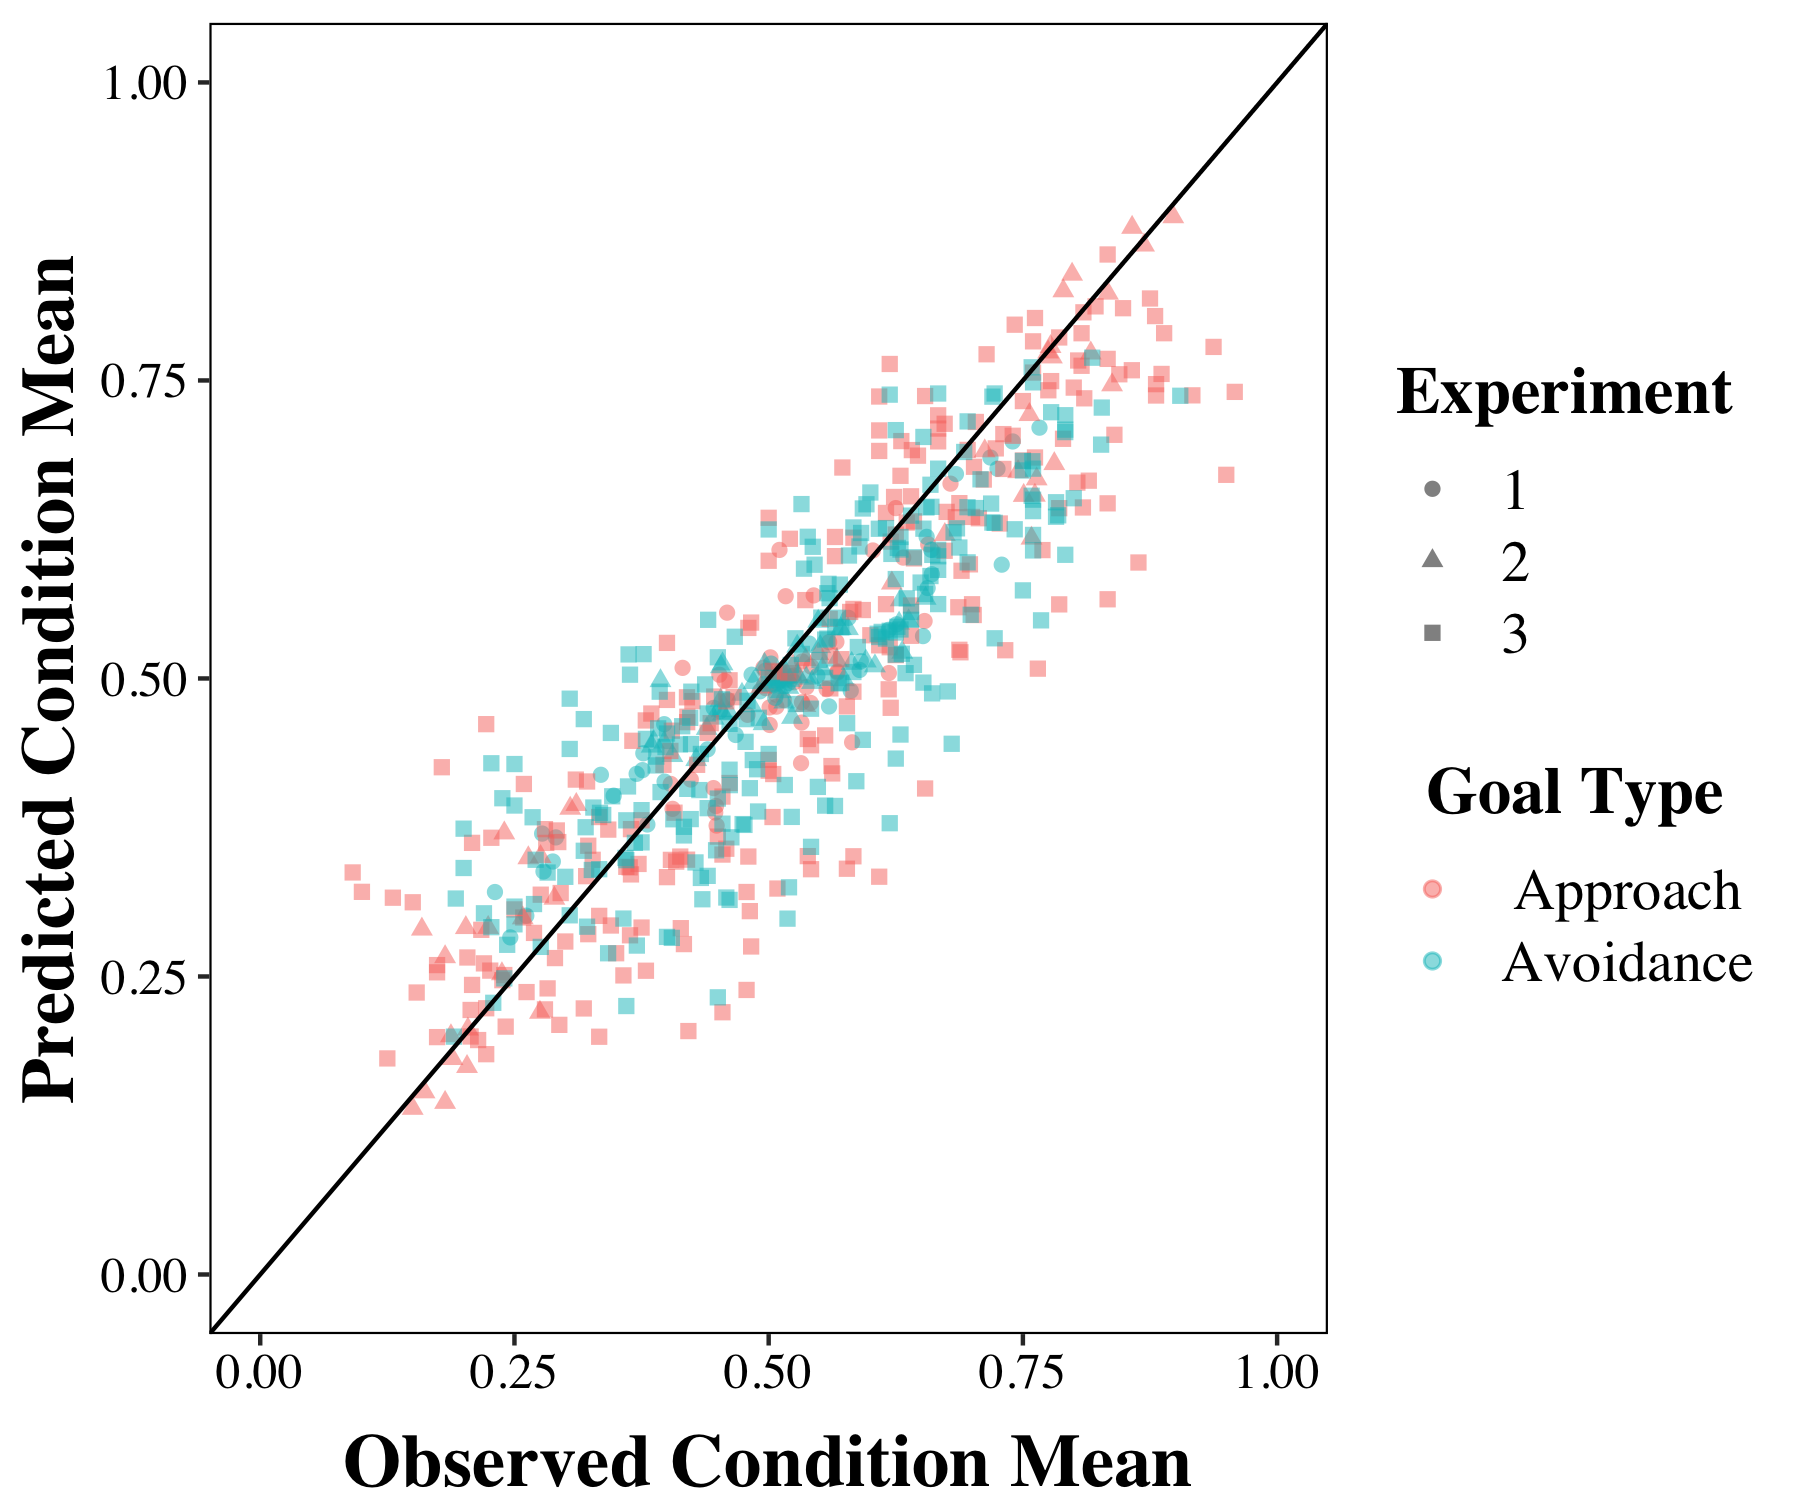
\includegraphics[width=0.8\textwidth]{predictives_scatterplot.png}
\caption{\label{fig:predictives_scatter} Relationship between observed and predicted mean proportions of decisions prioritizing the right-hand goal across the different trial configurations and goal type conditions in Experiments 1, 2, and 3. The condition means were computed by calculating the proportion for that trial for each participant and averaging across participants. This ensures that trials with more decisions did not exert a disproportionate influence on the mean value. }
\end{figure}

\subsection{Differences in Motivational Gradients between Approach and Avoidance}

We first consider the differences in the spatial, temporal, and spatiotemporal gradients between the approach and avoidance conditions. The goal of this analysis was to examine the extent to which each gradient influences the overall sense of motivation for the different types of goals. To do this, we computed the mean of the posterior distribution on each parameter for each participant and averaged this value across participants. This resulted in a single set of parameters for each goal type condition, which were used to model the strength of each gradient for different combination of distance to goal and time to deadline. The results of this analysis are presented in Figure \ref{fig:mean_gradients}. This figure is formatted in a similar manner to Figure \ref{fig:descriptives}, except that the vectors presented in Figure \ref{fig:mean_gradients} represent model generated gradients rather than observed data. In Figure \ref{fig:mean_gradients}, the length of the vector represents the strength of motivation attributable to each type of gradient.
% AJH Exactly how, I was assuming that the length of all three arrows would sum to a constant and correspond to the relative weights I defined above, but the sum just looks less in avoidance. Perhaps these are the un-normalized weights? I am not sure that is a good idea, I reckon this figure wants to show relativity's. Best do that and then just say in text (or show in supplement) the sums and comment on them in text ... although I am not intuting what they mean, if they were the same for left and right they would just become a mutiplier on the logistic, 1/(1+exp(S)*exp(-(Mright-Mleft)). As they are not I guess there is an elemnet in each of the total tendency to head right vs. left, so you migth best express this as 1/(1+exp(Ssum)*exp(-[S'right*M'right - S'left*M'left]) where S'i = Si/Sav and M' is the purely relatively weighted bit of the gradient sums). So actually this is good to, you get on number S'right = 1-S'left that expresses bias and Ssum that expresses the sharpness of the logistic to the tenency to make polarized choices (I think, just play with some numbers to figure it out).
%TB - I've updated the plots to show the normalised gradients. Note, however, that the avoidance gradients are still a bit smaller because the curvature parameter is such that they drop off more quickly in the avoidance condition than in the approach condition.
To simplify the presentation, the spatial dimension is broken down into six levels (0.125, 0.275, 0.425, 0.575, 0.725, and 0.875) and the temporal dimension is broken down into only low (0.1) and high (0.9) values.
%AJH Why 6 %TB - I chose six because it was enough that you could get a sense of the full pattern, but not so much that the plot appears too cluttered.

\subsubsection{Approach Condition}
In the approach condition (the left half of Figure \ref{fig:mean_gradients}),
% AJH isnt this already explained %TB - note quite. The meaning of the vector length is explained above, but the orientation needs an extra sentence because its meaning differs in approach (where the vectors point toward the thresholds) compared with avoidance (Where the vectors point away from the thresholds).
the extent to which the arrow points upward represents the strength of motivation to prioritize the left goal. The extent to which the arrow points rightward represents the strength of motivation to prioritize the right goal.
As expected the motivation attributable to the temporal gradient (shown in green) gets stronger when the deadline is closer. As can be seen in the top-left panel, where both goals have close deadlines, the temporal gradient is very strong for both goals, which is indicated by the long green arrows pointing diagonally upward and to the right. When one goal has a short deadline and the other has a long deadline, the temporal gradient favors the goal with the shorter deadline. When both goals have a long deadline, the temporal gradient is not influential at all, as indicated by green arrows being virtually absent in the bottom-right panel of the approach section.

The results for the approach condition suggest that the spatial gradient (shown in red) generally favors the goal that is closer to being achieved. This can be seen by the fact that the red arrows that are located above the diagonal tend to point upward whereas the red arrows that are below the diagonal tend to point rightward. The direction of motivation attributable to the spatiotemporal gradient (shown in blue) depends on both the distance to goal and the time to deadline. When both deadlines are close, the spatiotemporal gradient favors the goal that is closer to being achieved. This can be seen by the fact that the blue arrows in the top-left panel of the approach section of the figure align with the red arrows. When both deadlines are farther away, the spatiotemporal gradient favors the goal that is farther from being achieved. This can be seen by the blue arrows in the bottom-right panel of the approach section pointing inward towards the diagonal. These results suggest that the spatiotemporal gradient is strongest when the goal is moderately difficult to achieve.

\begin{figure}[h!]
\centering
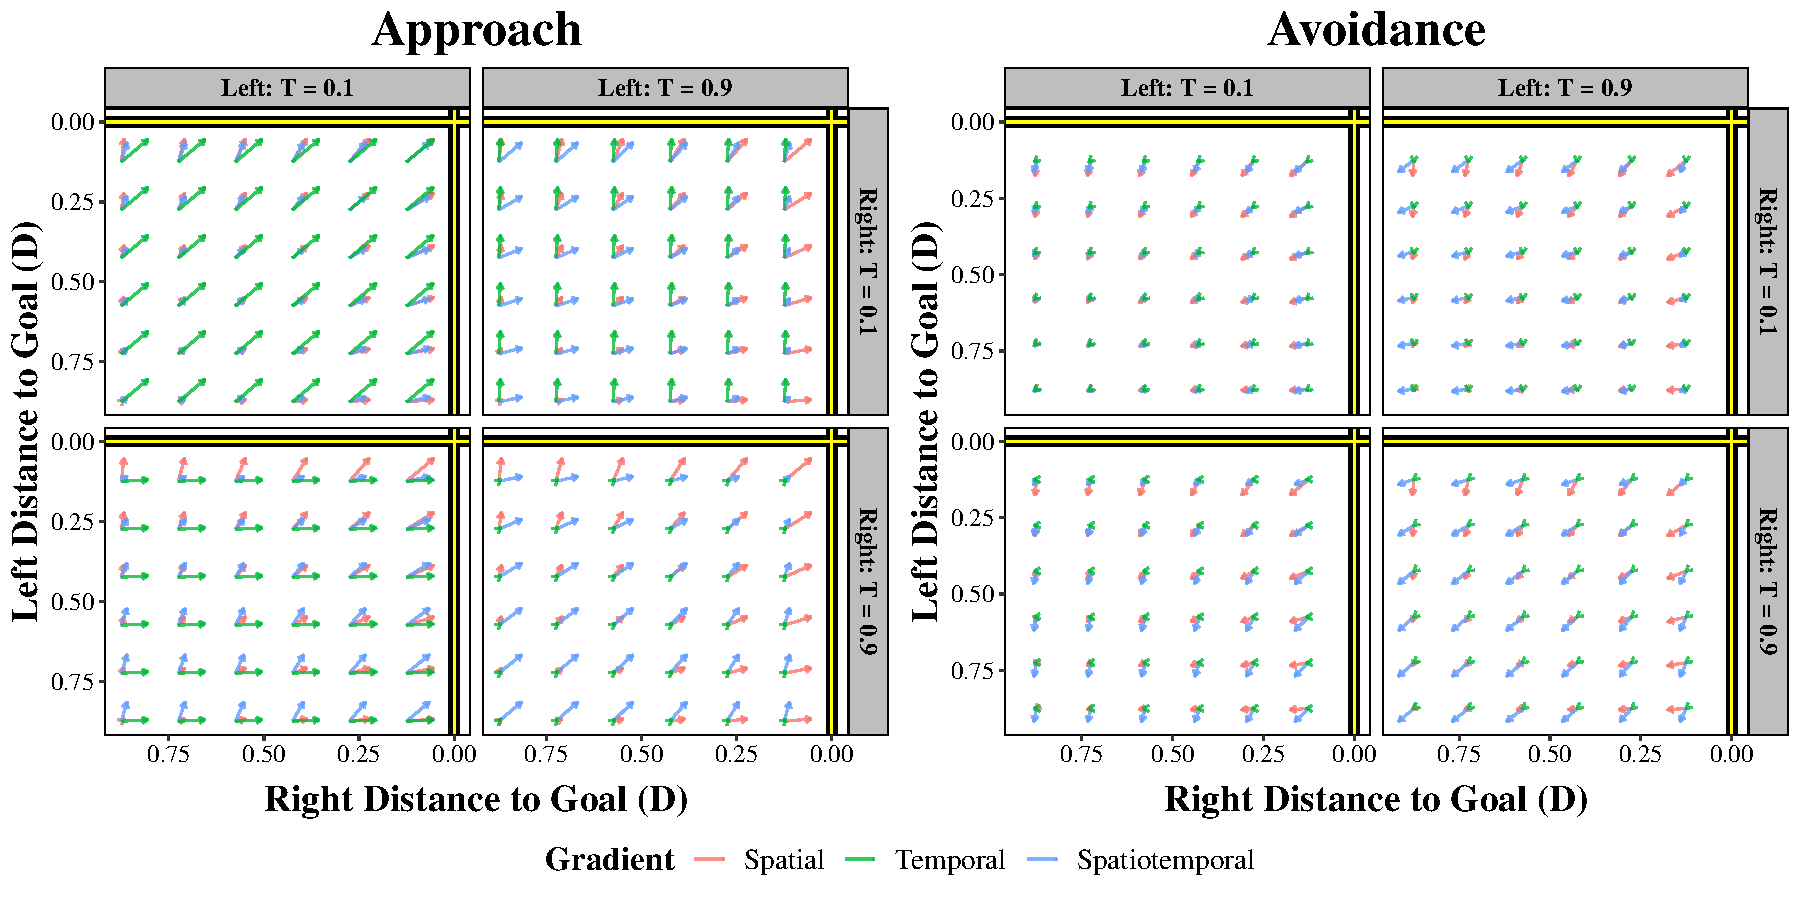
\includegraphics[width=1\textwidth]{mean_gradients_norm.pdf}
\caption{\label{fig:mean_gradients} The influence of distance to goal and time to deadline on the strength of the spatial (shown in red), temporal (green), and spatiotemporal (blue) gradients when pursuing approach and avoidance goals. Gradients were computed based on the average of the mean of the posterior distribution on each parameter for each participant. The length and orientation and of the vector indicate the strength and direction (respectively) of motivation implied by the gradients.}
\end{figure}

These results suggest that when pursuing approach goals, the relative influence of each gradient depends on the distances to the goals and the times to the deadlines. When one goal has a short deadline and the other has a long deadline (top-right or bottom-left panel of the approach section), the temporal gradient is dominant. Consistent with what we observed, this result suggests that the prioritization decision is primarily based on which goal has a shorter deadline. When both goals have a short deadline (top-left panel), the temporal gradients cancel out. However, in this case the spatial and spatiotemporal gradients are aligned -- both prefer the goal that is closer to being achieved. The alignment between the spatial and spatiotemporal gradients in this scenario explain the strong preference for prioritizing the closer goal when both deadlines are relatively short. When both deadlines are longer, the temporal gradients again cancel out, but in this scenario the spatial and spatiotemporal gradients are in conflict. The spatial gradient favors the goal that is closer to being achieved, but the spatiotemporal gradient favors the goal that is farther from being achieved. This explains the lack of clear prioritization preference when deadlines are farther away.

\subsubsection{Avoidance Condition}

In the avoidance condition, participants are motivated to move away from the undesired threshold. As expected based on the behavioral results, the temporal gradient has little to no influence in the avoidance condition. This can be seen by the virtual absence of green arrows in the right section of Figure \ref{fig:mean_gradients}. The results suggest that motivation when pursuing avoidance goals is mostly attributable to the spatial and spatiotemporal gradients. The spatial gradient increases in strength as the undesired threshold gets closer. The spatiotemporal gradient is strongest when either the undesired threshold is relatively far away but there is a lot of time remaining. This can be seen most clearly by the fact that the blue arrows in the bottom-right panel of the avoidance section are relatively long (particularly in the bottom-left corner of the panel where the distance to both thresholds is longer). These results suggest that the motivation to avoid is highest when either the undesired threshold is close (due to the spatial gradient) or when the threshold is farther away but a lot of time must be spent avoiding the threshold (due to the spatiotemporal gradient).

\subsubsection{Interim Summary}

The result thus far suggest that the spatial, temporal, and spatiotemporal gradients exert unique influences on motivation that help to explain the patterns of prioritization decisions observed in the three experiments. In the approach condition, the preference for prioritizing goals with shorter deadlines appears to be driven by the temporal gradient. The preference for prioritizing the closer of two goals with relatively short deadlines appears to attributable to the additive influence of the spatial and spatiotemporal gradients. Finally, the lack of a clear prioritization preference when goals have longer deadlines may be the result of conflict between the spatial and spatiotemporal gradients. In the avoidance condition, the tendency to prioritize the goal for which the undesired threshold is closer appears to have been driven primarily by the spatial and spatiotemporal gradients, with the temporal gradient exerting less influence in the avoidance context.

\subsection{Individual Differences in Motivational Gradients}

Having established the unique influences of the spatial, temporal, and spatiotemporal on motivation during goal pursuit, we next assessed the variability in these effects across individuals. To do this, computed each gradient separately for each participant and examined the influence of goal type, distance to goal, and time to deadline on the distributions of each gradient. The results of this analysis are presented in Figure \ref{fig:ids_in_each_gradient}. In this figure, each participant's gradient is shown as a partially transparent vector. The darker, thicker clusters of vectors represent gradients that are more common among participants.

\begin{figure}[h!]
\centering
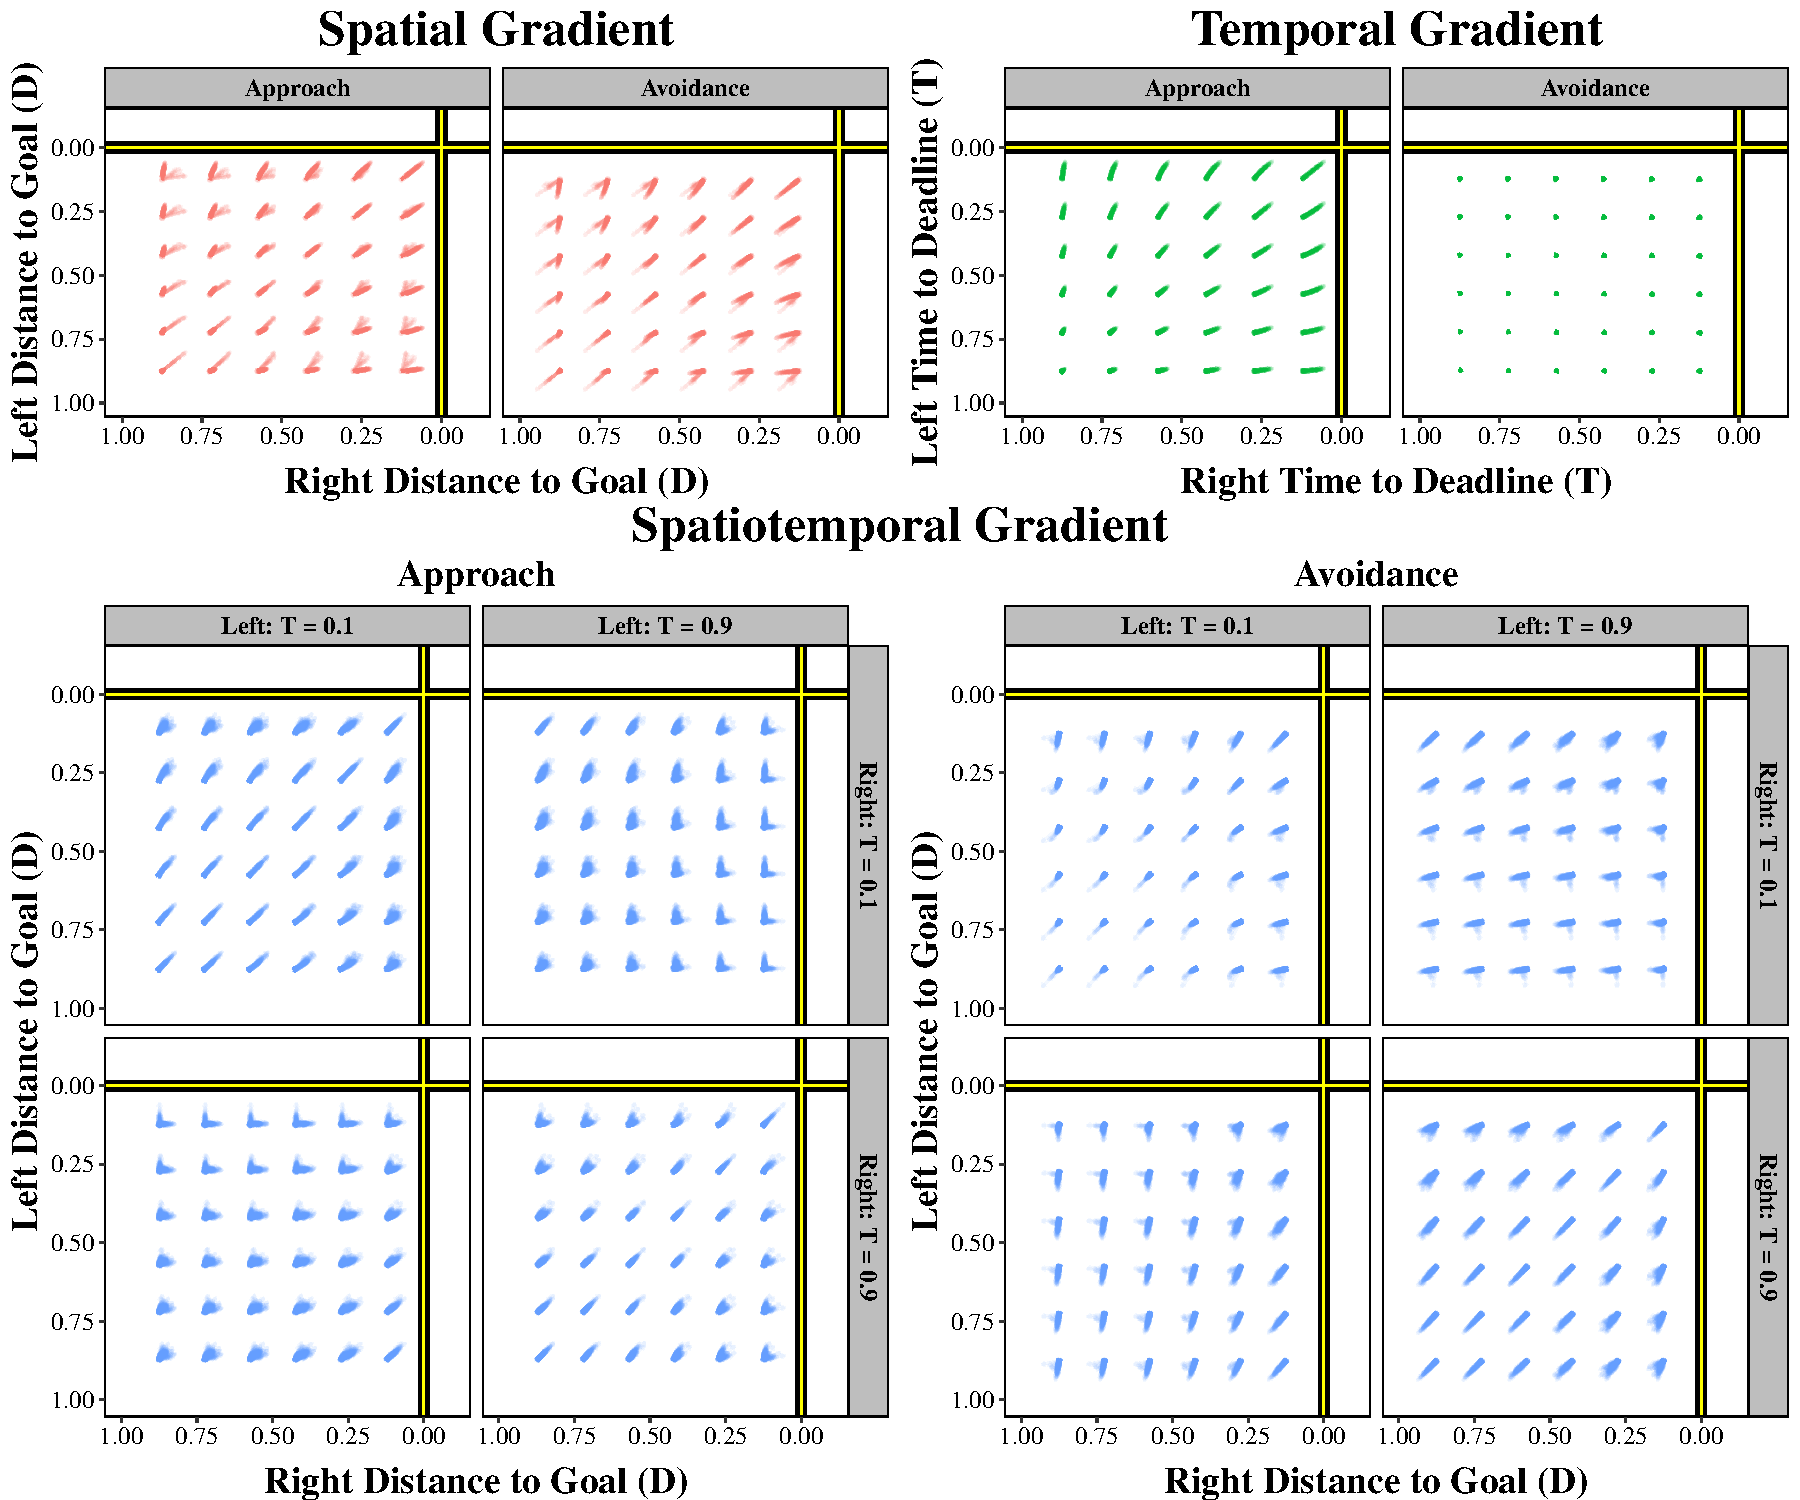
\includegraphics[width=1\textwidth]{ids_in_each_gradient_norm.pdf}
\caption{\label{fig:ids_in_each_gradient}  Individual differences in the influence of distance to goal and time to deadline on the strength of the spatial (shown in red), temporal (green), and spatiotemporal (blue) gradients when pursuing approach and avoidance goals. Gradients were computed based on the mean of the posterior distribution on each parameter for each participant. The length and orientation and of the vector indicate the strength and direction (respectively) of motivation implied by the gradients.}
\end{figure}


\subsubsection{Spatial Gradients}

The top-left section of Figure \ref{fig:ids_in_each_gradient} shows the influence of the distance to each goal on the spatial gradients for each participant. By definition, the spatial gradient is unaffected by time to deadline so this variable is not considered when assessing the spatial gradient. Consistent with the aggregated results presented in the previous section, the spatial gradient for most participants favors the goal that is closer. In the approach condition, this suggests that the spatial gradient drives most participants toward the goal with the closer threshold (i.e., the arrows point away from the diagonal toward the closer threshold). In the avoidance condition, the spatial gradient drives most participants away from the closer threshold (i.e., the arrows point toward the diagonal away from the closer threshold).

The individual differences in the spatial gradient depends on the distance to each goal. When both goals are relatively close to the threshold (seen in the top-right corner of each panel), the spatial gradients are relatively homogeneous. However, individual differences emerge when one goal is relatively close and the other is further away (seen in the top-left or bottom-right corner of each panel). In the approach condition, there is a subset of participants for whom the spatial gradient favors the goal that is further away. This subset is illustrated by the smaller cluster of vectors that point inward toward the diagonal. There also appears to be some evidence of a third subset in the approach condition for whom the spatial gradient favors both goals equally regardless of the distance to each goal. These participants have vectors that point diagonally upward and to the right.

In the avoidance condition, there do not appear to be any participants for whom the spatial gradient favor the goal for which the undesired state is further (i.e., there are no vectors that point inward toward the diagonal). However, there does appear to be a subset of participants for whom the spatial gradient favors both goals equally (i.e., vectors and that point diagonally downward and leftward).\footnote{It is important to note that these subsets are not accounted for by experiment. When the data are analyzed for each experiment separately, similar subsets emerge in each one. }

\subsubsection{Temporal Gradients}

The top-right section of Figure \ref{fig:ids_in_each_gradient} shows the influence of the time to each deadline on the temporal gradients for each participant. By definition, the temporal gradient is unaffected by distance to goal so this variable is not considered when assessing the temporal gradient. These findings suggest that influence of the temporal gradients is relatively homogeneous across individuals in both conditions. In the approach condition, the influence of the temporal gradients tend to strongly favor the goal with the shorter deadline (as indicated by the long vectors pointing toward the closer threshold). In the avoidance condition, the temporal gradients exert little to no influence on motivation (as indicated by the vectors being virtually absent in this condition).

\subsubsection{Spatiotemporal Gradients}

The bottom section of Figure \ref{fig:ids_in_each_gradient} shows the influence of distance to goal and time to deadline on the spatiotemporal gradients for each participant. As can be seen, the nature of the individual differences in the approach condition depend on both distance and time. Consider first the top-left panel in the approach section, where both goals have short deadlines. Along the positive diagonal, where both goals are the same difficulty, the spatiotemporal gradient favors the goals equally for all participants (as indicated by the diagonal vectors that point toward the top-right corner of the panel). However, individual differences emerge when one goal is closer to the threshold than the other (i.e., the top-left and bottom-right corners of the panel). Specifically, some participants have spatiotemporal gradients that favor the closer (i.e., easier) goal whereas others have gradients that favor the farther (i.e., harder) goal. The same pattern emerges in the bottom-right panel when both goals have longer deadlines.

A different pattern emerges when goals have different deadlines in the approach condition (the top-right and bottom-left panels). When the goal with the longer deadline is also a shorter distance to the threshold (i.e., top-left corner of the top-right panel, bottom-right corner of bottom-left panel), there is a large disparity in difficulty between the goals. The goal with the longer deadline and shorter distance is much easier to achieve than the the goal with the shorter deadline and longer distance. In this scenario, the spatiotemporal gradients are homogeneous--they tend to favor the two goals equally for all participants. When the goal with the longer deadline is also a longer distance to the threshold (i.e., bottom-right corner of the top-right panel, top-left corner of top-left panel), the goals are more similar in difficulty. In this scenario, the individual differences are more pronounced. These results together suggest that in the approach condition, individual differences in the spatiotemporal gradient are most pronounced when the difference in difficulty between the two goals is relatively modest (without being so small as to render the spatiotemporal gradient irrelevant).

In the avoidance condition, as can be seen, there are fewer individual differences in the spatiotemporal gradient. The aggregated results presented in the previous section appear to accurately reflect the behavior of most participants.

\subsubsection{Interim Summary}

The findings presented in this section suggest that the ways in which goals induce motivation differ across individuals. The nature of these individual differences depends on several factors. First, the nature of these individual differences depend on the type of goal. Our results suggest that there is more variation when pursuing approach goals than avoidance goals. Second, the nature of this variation differs across the three gradients. Our results suggest that there is more variation between individuals in the spatial and spatiotemporal gradients than there is in the temporal gradient. Finally, the nature of the individual differences depend on the distance to each goal and the time to each deadline. Our results suggest that individual differences are most pronounced when these factors are such that there is a modest difference in difficulty between the goals being pursued.

\subsection{Overall Motivational Value}

In the previous sections, we used the GOAL architecture to determine the direction of motivation under different conditions in the experimental task. We found that the underlying spatial, temporal, and spatiotemporal gradients helped to explain participants' choices regarding which of two goals to prioritize. We now consider the more general question of how the distance to goal and time to deadline influence the overall extent to which approach and avoidance goals are motivating. To answer this question, we used the parameters estimated by the GOAL architecture to compute the spatial, temporal, and spatiotemporal gradients for a single, hypothetical goal. We use this information to evaluate the evidence for the six perspectives on motivation during goal pursuit described in the introduction.

The results of this analysis are presented in Figure \ref{fig:gradients}. The top row of the figure shows how distance to goal and time to deadline influence the overall motivational value, which represents the sum of the effects of the spatial, temporal, and spatiotemporal gradients. The results suggest that the overall motivational value of an approach goal changes in response to both distance to goal and time to deadline. The motivational value is higher when the goal is relatively close to being achieved and when the deadline is relatively near (i.e., the bottom-left corner of the panel), and decreases as either distance to goal or time to deadline increases. This overall pattern of results is not consistent with any of the six perspectives shown in Figure \ref{fig:Gradients}.

The results also suggest that the motivational value of an avoidance goal changes primarily in response to the distance to the goal. Motivation to avoid is highest when the goal is relatively close (i.e., when the undesired state is near; shown in the left side of the panel) and decreases as the distance to goal increases. As can be seen, the influence of time to deadline on the motivational value of an avoidance goal is relatively weak. This overall pattern is most consistent with the proximity perspective.

\begin{figure}[h!]
\centering
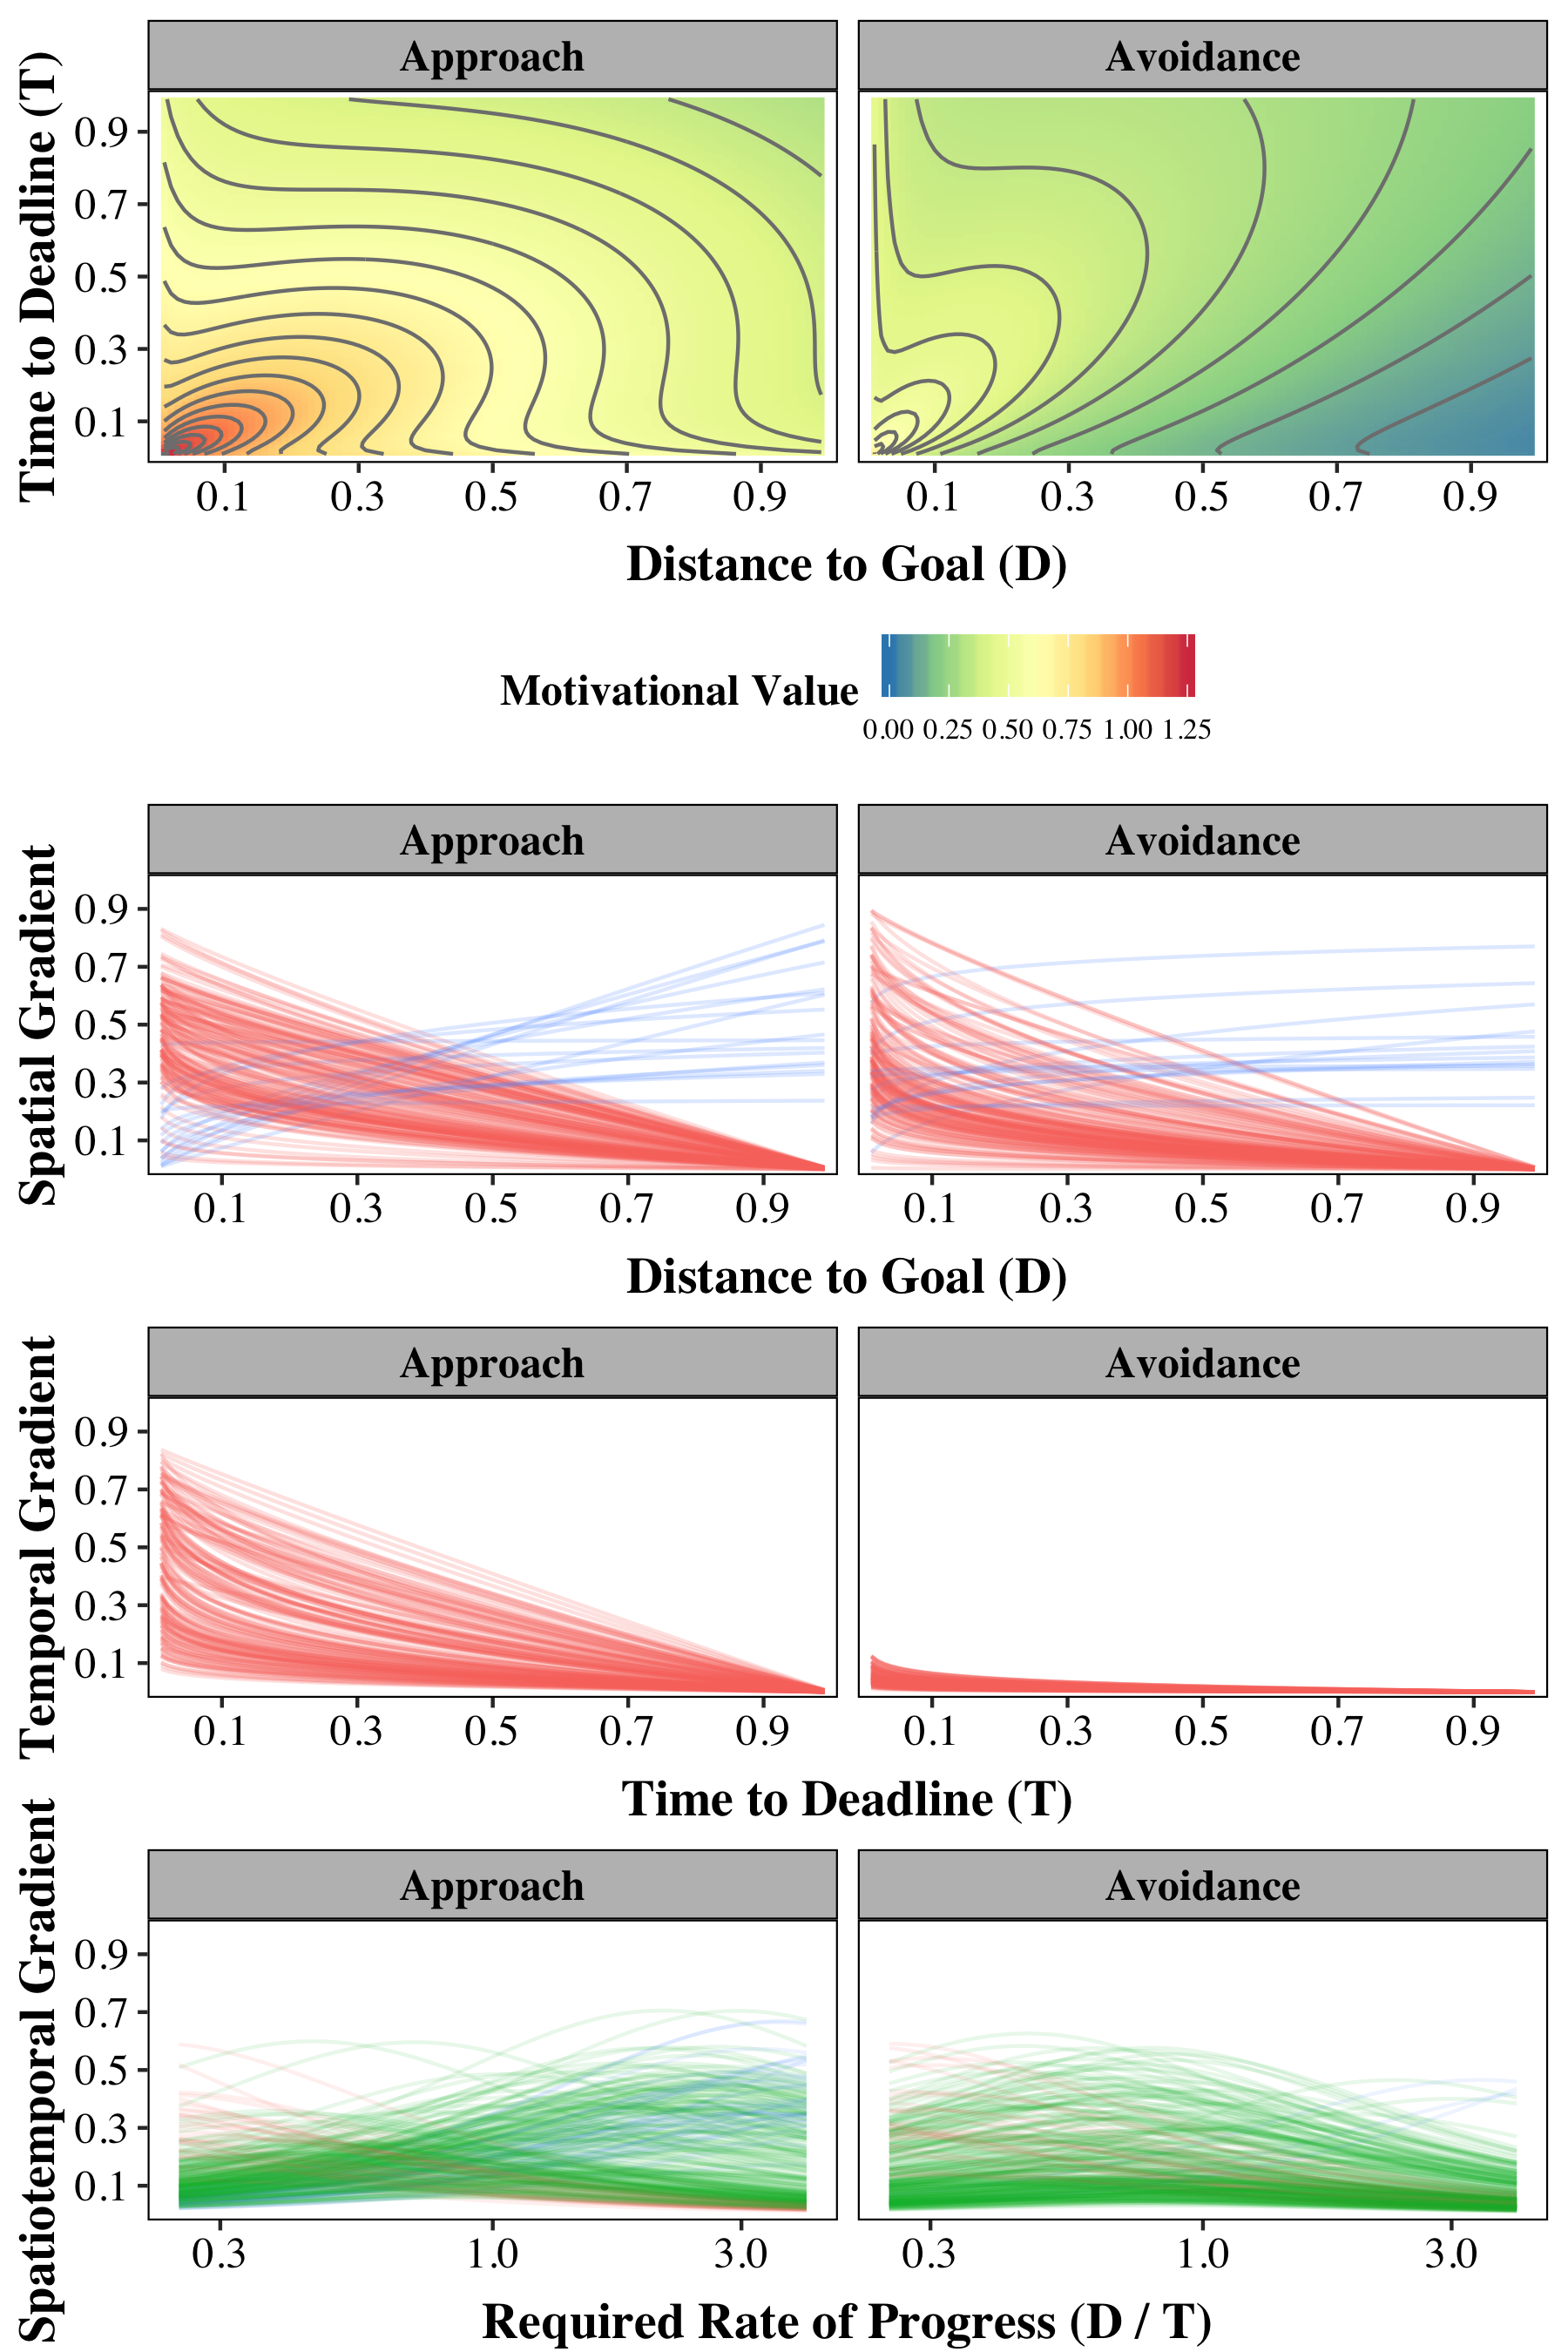
\includegraphics[width=0.9\textwidth]{overall_motivation.png}
\caption{\label{fig:gradients} Estimated overall motivational value (top row) and spatial (second row), temporal (third row), and spatiotemporal (bottom row). The motivational value shown in the surface plots represents the predictions implied by the mean of each participant's posterior mean. Spatial, temporal, and spatiotemporal gradients are shown for each participant, and represent the predictions implied by the posterior means for the relevant parameters. Spatial or temporal gradients that are a decreasing function of distance to goal or time to deadline are shown in red. Gradients that are an increasing function are shown in blue. Spatiotemporal gradients that are monotonically increasing on the interval (0.35, 3.5) are shown in blue. Those that are monotonically decreasing on that interval are shown in red. Spatiotemporal gradients that are non-monotonic on that interval are shown in green.}
\end{figure}

The second, third, and fourth rows of Figure \ref{fig:gradients} show the contribution of the spatial, temporal, and spatiotemporal gradients to the overall motivational value. The second row shows the spatial gradients, which were calculated based on the posterior means for the $w_1$ and $\delta$ parameters for each participant in Experiments 1 and 3. Gradients that are a decreasing function of distance to goal (consistent with the proximity perspective) are shown in red, whereas gradients that increase with distance to goal (consistent with the discrepancy perspective) are shown in blue. In both approach and avoidance goals, the majority of the gradients decrease with distance to the goal (89.4\% in approach, 92.8\% in avoidance), which provides evidence in favor of the proximity perspective.

The third row shows the temporal gradients, which were calculated based on the posterior means for the $w_2$ and $\tau$ parameters for each participant in Experiments 2 and 3. The temporal gradients differ approach and avoidance goals. The results suggest that the temporal gradients for approach goals are relatively steep, and are generally steeper than the spatial gradients for approach goals. By contrast, the temporal gradients for avoidance goals are flat. This finding suggests that when pursuing approach goals, the temporal gradient may be more influential than the spatial gradient, whereas when pursuing avoidance goals, the spatial gradient is likely the more influential of the two.

The fourth row shows the spatiotemporal gradients, which were calculated based on the posterior means for the $w_3$ and $\alpha$ parameters for each participant across all three experiments. The x-axis for these panels represents the rate of progress required to reach the goal, which corresponds to the ratio of the distance to goal and time to deadline. We classified participants' gradients as being increasing, decreasing, or non-monotonic functions of the required rate of progress by considering the monotonicity of the gradient on the interval (0.35 , 3.5). This interval was chosen because it represents approximately the 10th and 90th percentiles of the distribution of required rates encountered by participants in the experiments. This means that participants with monotonic spatiotemporal gradients on this interval were most motivated by goals that were either among the easiest to achieve (consistent with the expectancy perspective) or among the hardest to achieve (consistent with the difficulty perspective).

As can be seen, there was variation in the nature of the spatiotemporal gradient between individuals in the approach condition. In this condition, 79.6\% of participants had non-monotonic gradients (shown in green), suggesting that there were more motivated that required a moderate rate of progress in order to achieve. 11.6\% of participants had spatiotemporal gradients that decreased with the required rate of progress (shown in red), suggesting that they were most motivated by the goals that were easiest to achieve. 8.8\% of participants had gradients that increased with the required rate (shown in blue), suggesting that they were most motivated by the hardest goals. These findings suggest that the non-monotonic perspective is sufficient to account for the spatiotemporal gradients for most individuals, but that the expectancy and difficulty perspectives are both needed to account for the full extent of variation when pursuing approach goals.

In the avoidance condition, the spatiotemporal gradients tended to be weaker than in the approach condition. 88.1\% of participants had non-monotonic spatiotemporal gradients in this condition. 11.2\% had gradients that decreased with the required rate. In the avoidance condition, a decreasing gradient indicates that motivation is highest for the hardest goals (i.e., goals for which it is easy to reach the undesired state). Only 0.7\% (N=2) of participants in the avoidance condition had gradients that increased with the required rate of progress. These findings suggest that most people can be accounted for by the non-monotonic perspective, but that there is a subset of individuals who are better described by the difficulty perspective in the avoidance condition.

These results together reinforce the conclusion that there is diversity in the ways in which goals influence motivation across both individuals and goal types. Approach goals appear to influence motivation via all three gradients. This finding suggests that none of the perspectives described in the introduction is sufficient to account for the dynamics of approach goal pursuit in its own right. It appears that the proximity perspective, the temporal perspective, and the non-monotonic perspective are all necessary to explain these dynamics for most individuals. Avoidance goals appear to influence motivation primarily via the spatial gradient. The results suggest that the proximity and discrepancy perspectives (which make the same predictions in the avoidance context) may be sufficient to account for the dynamics of motivation during avoidance goal pursuit. However, there was also evidence that, for some individuals, the spatiotemporal gradient contributes to avoidance goal pursuit. This suggests that the non-monotonic perspective (and to a lesser extent the difficulty and expectancy perspectives) may also be necessary to explain the dynamics of motivation in the avoidance context.


\section{Normative Modeling Results}

In the final set of analyses that we report, we shift focus from the question of how people prioritize goals to the question how \textit{well} people prioritize goals. To answer this question, we examine the extent to which participants' decisions in the three experiments aligned with a normative model of decision making that maximized the number of goals achieved in this task. We calculated the normative decisions using dynamic programming \citep{Hutchinson2000}. The normative model assumed that, after each trial, end-states in which both goals were achieved had a value of two, end-states in which only one goal were achieved had value of one, and end-states in which neither goal had been achieved had no value. The normative model also assumed that the values of the possible end-states were not discounted over time. For every decision point encountered by each participant in the three experiments, the normative model identified the decision that would maximize the expected number of goals achieved. This model therefore provided a benchmark by which evaluate the effectiveness of participants' decisions in this task.

Overall, participants made better decisions when pursuing approach goals compared with when pursuing avoidance goals. Participants' prioritization decisions matched the normative model's decision 62.7\% of the time in the approach condition, but only 53.2\% of the time in the avoidance condition. There was also considerably more variation between participants in decision effectiveness when pursuing approach goals (standard deviation of proportion of decisions aligning with normative model = 0.11) compared with avoidance goals (sd = 0.06). The extent to which participants decisions aligned with the normative model also depend on the distances to the goals and times to each deadline. Figure \ref{fig:normative_gradients} shows the influence of these factors on the decisions generated by the normative model. The colour of the vectors in Figure \ref{fig:normative_gradients} represents proportion of participants' decisions that align with the normative model. As can be seen, in the approach condition, the normative model generally prioritizes the goal that is closer to being achieved when the two goals have short deadlines...

THE MAIN TAKEAWAY FROM THIS SECTION WOULD BE THAT IN THE APPROACH CONDITION, PEOPLE ARE PARTICULARLY "OPTIMAL" WHEN AT LEAST ONE DEADLINE IS SHORT (THIS IS WHERE THERE ARE THE MOST RED ARROWS), BECAUSE GENERALLY IN THIS SITUATION THE OPTIMAL CHOICE IS TO PRIORITIZE THE GOAL WITH THE CLOSER DEADLINE. THAT SAID, WHEN THE OPTIMAL DECISION IS TO PRIORITIZE THE GOAL WITH THE LONGER DEADLINE, PEOPLE ARE QUITE POOR. THIS SUGGESTS THAT THEY DO NOT LIKE TO ABANDON THE GOAL WITH THE CLOSER DEADLINE. IN THE AVOIDANCE CONDITION, PEOPLE STRUGGLE MOST WHEN GOALS HAVE DIFFERENT DEADLINES. THIS IS BECAUSE THEY DO NOT PAY ATTENTION TO DEADLINE. SO THE SOMEWHAT INTERESTING TAKEAWAY IS THAT PEOPLE MIGHT OVERWEIGHT DEADLINE INFORMATION WHEN PURSUING APPROACH GOALS AND UNDERWEIGHT DEADLINE WHEN PURSUING AVOIDANCE GOALS. THAT SAID, I DON'T THINK THIS RELATIONSHIP IS IMMEDIATELY OBVIOUS FROM FIGURE 7. AND IN GENERAL THE NORMATIVE MODELLING SECTION FEELS TACKED ON. SO I'M NOT SURE IF ITS WORTH INCLUDING.


\begin{figure}[h!]
\centering
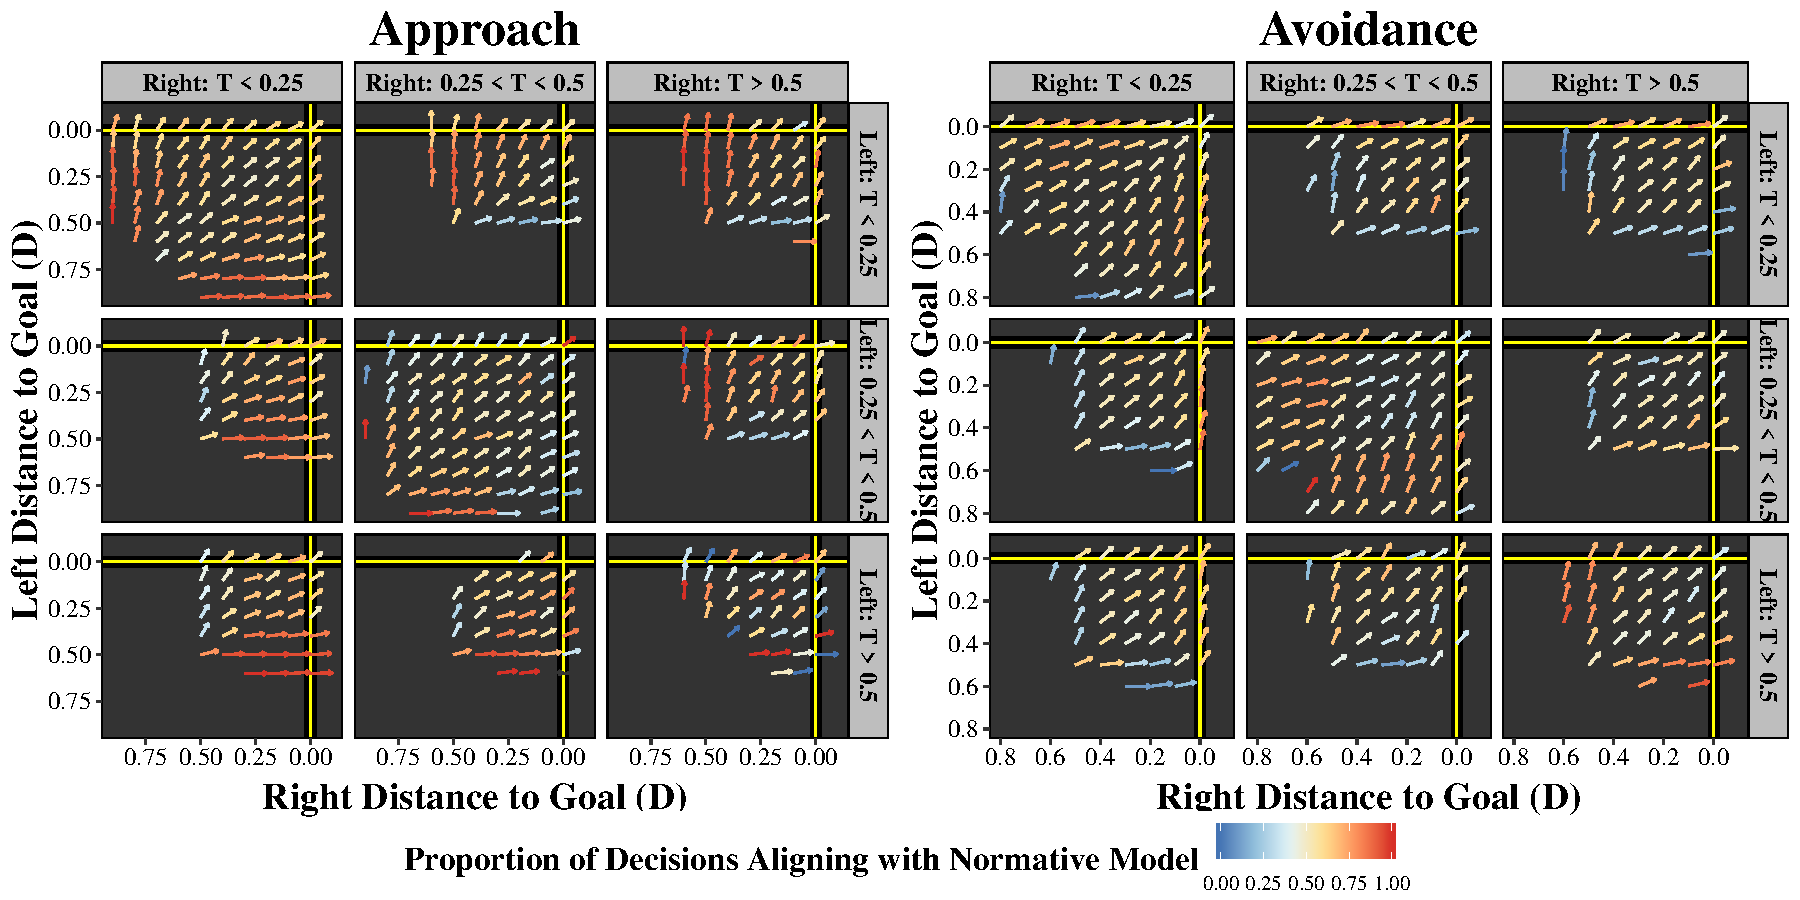
\includegraphics[width=0.9\textwidth]{normative_gradient.pdf}
\caption{\label{fig:normative_gradients} Insert text here...}
\end{figure}


\section{General Discussion}

Although attempts to understand how motivation changes over time as a person pursues a goal have a long history in psychology, progress in this area has been limited due to the proliferation of bespoke theories that are narrow in focus and that often make conflicting predictions. We identified six theoretical perspectives that could be used to generate predictions regarding the dynamics of motivation when pursuing approach and avoidance goals (see Figure \ref{fig:hypothetical_gradients}). Two perspectives--the proximity and discrepancy perspectives--propose that motivation changes with the distance to the goal (i.e., the amount of progress needed to reach it), but do not consider the effects of deadlines. One perspective proposes that motivation changes with the amount of time available before the deadline, but does not consider the effects of distance to the goal. Finally, three perspectives consider how the difficulty of the goal might influence motivation, but do not explicitly consider either distance or time.

The GOAL architecture integrates these diverse perspectives and provides a framework for comparing them. The GOAL architecture assumes that the motivation to prioritize a goal is influenced by three gradients. The spatial gradient represents the changes in motivation that are due to changes in the distance to the goal. The temporal gradient represents the changes in motivation that are due to the looming deadline. The spatiotemporal gradient represents the changes in motivation that are attributable to the ratio of the distance to the goal to the time to the deadline (i.e., the rate of progress required to reach the goal) and captures the effects of goal difficulty on motivation.

We used the GOAL architecture to quantify the three gradients by fitting the model to participants' goal prioritization decisions from three experiments. The results revealed considerable diversity across situations and individuals in the ways in which the gradients influenced motivation. When pursuing approach goals, all three gradients were influential but the temporal gradient tended to be the strongest. However, there was a great deal of variation between individuals in the effects of the spatial and spatiotemporal gradients. For most participants, the spatial gradient was negative, indicating that motivation increased as the individual moved closer to the goal and providing support for the proximity perspective. However, there were some participants for whom the spatial gradient was positive in line with the discrepancy perspective. Moreover, although the spatiotemporal gradient was non-monotonic for most people, there were subsets of individuals whose decisions were more consistent with the difficulty and expectancy perspectives. These findings together suggest that none of the six existing theoretical perspectives is sufficient to account for the dynamics of approach goal pursuit in its own right. Our results suggest that the temporal gradient, the proximity perspective relating to the spatial gradient, and the non-monotonic perspective relating to the spatiotemporal gradient are all required to account for the behavior of most individuals when pursuing approach goals.

In contrast to the approach context, when pursuing avoidance goals, the spatial gradient was the strongest and the temporal gradient exerted almost no influence. Furthermore, there was less heterogeneity across individuals in the effects of each gradient. For most participants, the spatial was negative indicating that motivation increased as the individual moved closer to the undesired state. These results are in line with both the proximity and discrepancy perspectives, which make the same predictions in the avoidance context. We also found that the spatiotemporal gradient was influential for some individuals in the avoidance context, with most individuals displaying non-monotonic gradients but some having gradients that were more consistent with the difficulty perspective. However, the influence of the spatiotemporal gradient was generally weaker than in the approach context. These results suggest that the spatial gradient might be sufficient to account for the behavior of most individuals when pursuing avoidance goals, but that the non-monotonic and difficulty perspectives relating to the spatiotemporal gradient may also be required for certain individuals.

\subsection{A Linking Architecture}

The GOAL architecture has the potential to help bridge the gap between theories of motivation and models of decision making, which will open up new areas for future investigation. For example, models of choice and response time such as the diffusion decision model \citep[DDM;][]{Ratcliff2018a,Ratcliff1978,Ratcliff2008} and the linear ballistic accumlator model \citep[LBA;][]{Brown2008} consider the dynamics that play out within a single decision episode. These models assume that people make decisions by accumulating evidence in favor of possible courses of action until the evidence for one alternative breaches a threshold, at which point that action is selected. However, research that has applied these models has typically only examined independent, one-shot decisions. This research therefore fails to capture the inter-decision dynamics that play out across a series of interdependent decisions, such as those involved in goal pursuit.

The GOAL architecture can be integrated with models like the DDM and LBA to investigate these dynamics. This can be achieved by using the GOAL architecture as a front-end model that links the spatial, temporal, and spatiotemporal gradients to different components of the decision making process. For example, people tend to set lower thresholds when under time pressure, such that they require less evidence to make a decision \citep{Ratcliff1998,Pleskac2018,Usher2001,Rae2014}. This finding suggests that people should make less cautious decisions when confronted by a looming deadline. However, there are multiple ways in which deadlines might exert an effect. One possibility is that people adjust their response caution according to the time remaining, which would imply that the threshold is influenced by the temporal gradient. An alternative account is that caution is determined by the rate of progress required to achieve the goal before the deadline, which would imply that threshold is influenced by the spatiotemporal gradient. It is also possible that these gradients might also influence the speed with which people process information, as previous research has found evidence for a relationship between time pressure and the rate of evidence accumulation \citep{Rae2014,Palada2018}. The GOAL architecture provides a framework that can answer these types of questions, and in doing so, help to elucidate the mechanisms by which motivation and decision making interact.

This architecture also has the potential to enhance our understanding of risky decision making. Prospect theory describes how reference points influence the preference for risky decision alternatives. People generally prefer risky alternatives when in the domain of losses (i.e., when below the reference point) and safer alternatives when in the domain of gains (i.e., when above the reference point). Some have used this theory to make predictions about the effects of goals or aspiration levels on motivation and decision making \citep[e.g.,][]{Heath1999,Wang2012a}. This research generally assumes that the extent to which people are willing to exert effort or take risks in order to achieve the goal is a function of the distance to the reference point. These theories, however, fail to consider the effects of time. Our research indicates that goals are evaluated differently depending on the temporal proximity of the deadline. This suggests that an integration between the GOAL architecture and prospect theory-based accounts of goal pursuit might be enable a more comprehensive account of the ways in which goals influence risky decision making.

Another area in which the GOAL architecture could help further our understanding is the literature that has examined the cognitive cost of effort \citep[e.g.,][]{Westbrook2013,Westbrook2015}. This research that has shown that, given two options that are equally rewarding, people tend to choose the one that requires less work \citep{Kool2010,Inzlicht2018}. This principal has come to be known as the ``law of less work''. Indeed, in many cases, people prefer the option that requires less work even when that option is less rewarding \citep[a phenomeon known as ``effort discounting'';][]{Botvinick2009,Libedinsky2013}. Although this research has revealed much about the relationship between rewards and effort, studies in this literature typically do not consider the effects that goals and deadlines have on the willingness to engage in a cognitively demanding task. According to the GOAL architecture, the willingness to exert effort should not only be a function of the reward, but also a function of the amount of time one has available and the length of time the effort must sustained in order to achieve the goal. These insights can be used to generate new predictions regarding how people regulate cognitive effort.

The GOAL architecture also provides a framework for linking behavioural measures of motivation to physiological data that captures the underlying neural mechanisms \citep[e.g.,][]{Turner2016,Palmeri2017,Palestro2018}. Evidence suggests that approach and avoidance motivation are instantiated in separate brain regions \citep{Wager2003,Rutherford2011}. There are a number of ways in which measures of brain activity in these regions (e.g., via EEG or fMRI) could be integrated with the GOAL architecture. One way would be examine the correlation between these measurements of brain activity and the strength of each gradient in order to elucidate the nueral processes underlying each one. Another method would be to fit the model directly to the neural activity measures, so that the estimated gradients are informed by both the behavioural and neural data. (THIS PROBABLY NEEDS FLESHING OUT).

\subsection{Capturing the Process}

Although we believe the GOAL architecture has the potential to further our understanding of motivation and decision making, it is important to recognize its limitations. The model is a descriptive, algebraic model that makes no assumptions about the underlying information processing that gives rise to a goal having motivational value. It takes time for a person to form a judgement of how far they are from reaching the goal and how much time is available and to then integrate this information. An understanding of how this process plays out could be useful for constraining the predictions of the GOAL architecture. Theories of multi-attribute decision making  \citep{Roe2001,Noguchi2018,Trueblood2015,Bhatia2013,Usher2004} may offer insight into how people process goal-related information. These theories generally assume that preference for a particular course of action accumulates over time as people shift attention between the different attributes, evaluating the options on each one. It is possible that people process information regarding the distance to the goal and the time to the deadline in a similar manner. Future research that seeks to test these assumptions might also benefit from using process-tracing methods, which can help to further clarify how information is being processed \citep{Schulte-Mecklenbeck2017}.

A unique feature of decision making during goal pursuit that is not generally relevant to other multi-attribute decisions is the sequential, interdependent nature of the choices being made. In this context, the distance to the goal and the time to deadline change in a predictable manner across the sequence of decisions. We would therefore expect to observe longer response times for the first decision in each goal pursuit episode (before which the distance to goal and time to deadline are unknown) compared with downstream decisions in the same episode. This decrease in response time could be accounted for by a model that assumes that the information accumulated about distance and time carries over from one choice point to the next. However, another possibility is that people do not necessarily make a new decision each time they produce a response. Instead, they might select a course of action at the first decision point and keep executing that same action across subsequent decisions until some stopping rule is reached (e.g., the required rate of progress exceeds some maximum value). Further research will be needed to understand the nature of these sequential dependencies in the decisions that are made during goal pursuit.

A model that captures how people process goal-related information will also help us understand the ways in which this process might change when people experience time pressure or capacity limitations. The principle of bounded rationality assumes that people have limited information processing resources and therefore often must rely on relatively simple decision rules or heuristics, particularly when time or capacity is limited \citep{Simon1956,Gigerenzer1996}. In the context of goal pursuit, one strategy might be to simply prioritize the goal with the shortest deadline. An alternative would be to prioritize the goal that is closest to being reached. We might also expect people to rely on simpler rules or heuristics when the number of goals being pursued is greater. This is because the presence of additional goals to consider would increase the complexity of the computations required to integrate and compare information regarding distance and time across the goals. At some point, the computations required will exceed the capacity of the individual, which should prompt a shift to a simpler strategy.

%other issues that could be discussed - uncertainty in deadlines/distance. %Incentives?

\section{Conclusions}

TBD


\clearpage
\bibliography{library}
\clearpage

\appendix
\section{}
\begin{figure}[h!]
\centering
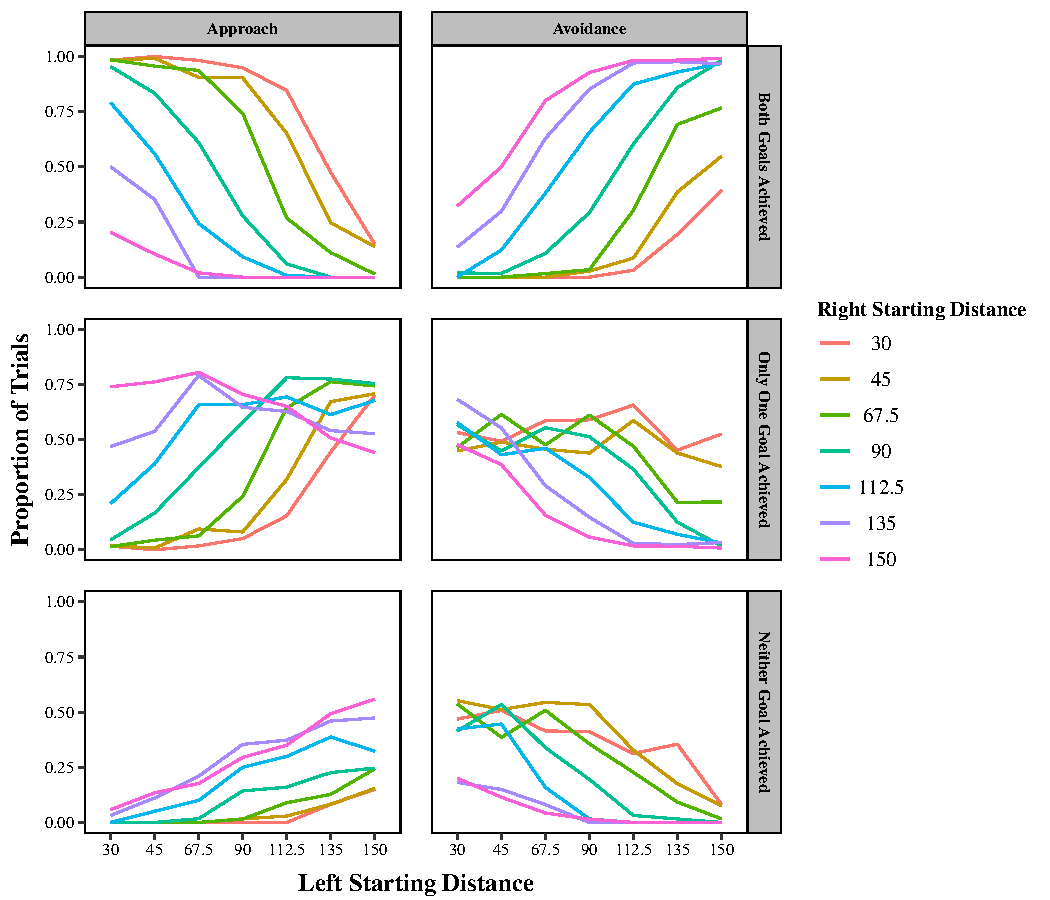
\includegraphics[width=1\textwidth]{GoalAchievement-Distance.pdf}
\caption{\label{fig:GoalAch-Distance} Rates of the different goal achievement outcomes as a function of goal type and starting distance in Experiment 1.}
\end{figure}

\clearpage
\section{}
\begin{figure}[h!]
\centering
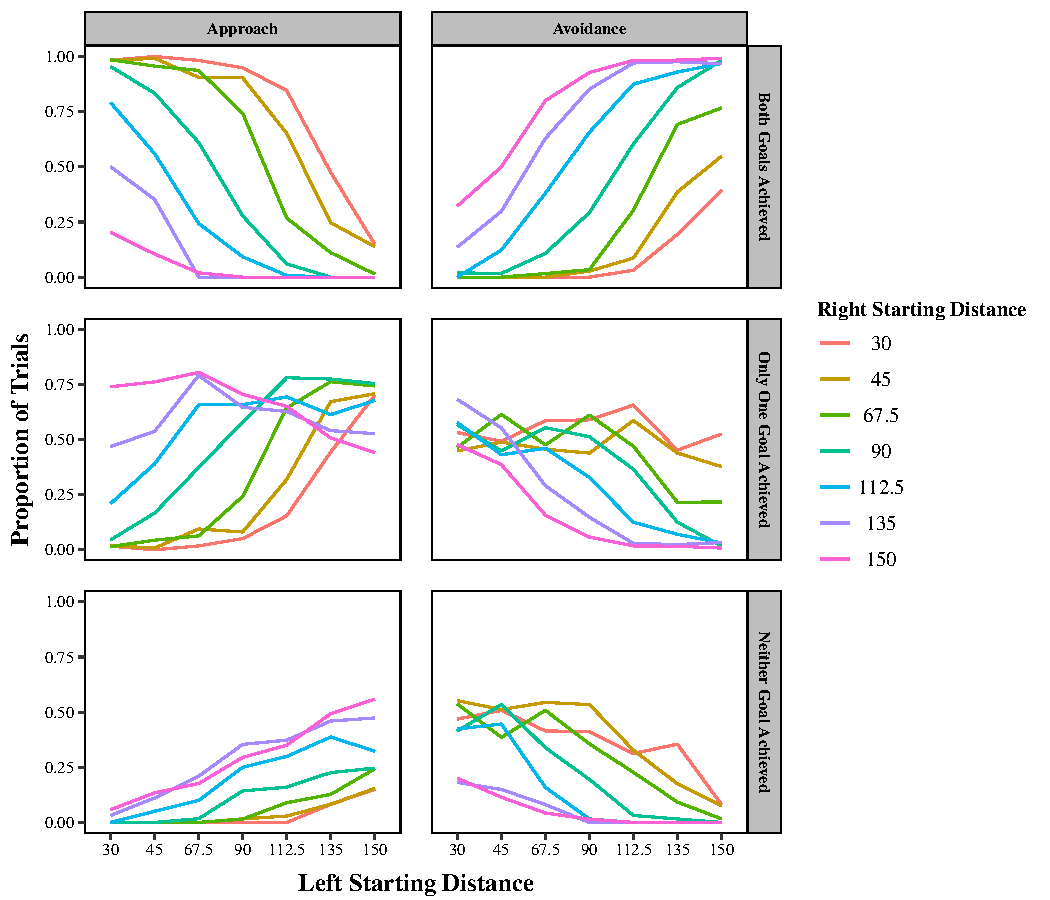
\includegraphics[width=1\textwidth]{GoalAchievement-Distance.pdf}
\caption{\label{fig:GoalAch-Deadline} Rates of the different goal achievement outcomes as a function of goal type and deadline in Experiment 2.}
\end{figure}

\clearpage
\section{}

%Details on priors and how the model was calculated the gradients.

The priors were chosen to be weakly informative. Parameters that were constrained to be positive had priors that were log-normally distributed. Parameters that were constrained to be negative also had log-normally distributed priors, but were multiplied by $-1$ before being applied. In models where the alpha parameter was estimated, it was constrained to between 0 and 1 using a beta distributed prior. The hyperpriors for the mean-log parameters were vague and normally distributed. The hyperpriors for the sd-log and beta parameters were log-normally distributed. The likelihood function was calculated by transforming the difference in motivation for the right and left goals into a choice probability via a logistic transformation.
%AH and I originally discussed a probit transform. This is certainly possible but takes longer, so I've been using a logistic instead.

\end{document}

%
% Please see the package documentation for more information
% on the APA6 document class:
%
% http://www.ctan.org/pkg/apa6
%
